% appendix

\chapter{公式总结}

% extra formulas

\section{三角复习}

\subsection{弧度制}

\begin{itemize}
    \item 定义:
    \begin{equation*}
        \textrm{弧度}=\frac{\textrm{弧长}}{\textrm{半径}}
    \end{equation*}
    \item 特殊值:
    \begin{center}
        \renewcommand\arraystretch{1.2}
        \begin{tabular}{c|c|c|c}
            \hline
            角度&弧度&角度&弧度\\\hline
            $30^\circ$&$\pi/6$&$120^\circ$&$2\pi/3$\\
            $45^\circ$&$\pi/4$&$135^\circ$&$3\pi/4$\\
            $60^\circ$&$\pi/3$&$150^\circ$&$5\pi/6$\\
            $90^\circ$&$\pi/2$&$180^\circ$&$\pi$\\
            \hline
        \end{tabular}
    \end{center}
\end{itemize}

\subsection{三角函数}

\begin{itemize}
    \item 正弦:对边/斜边
    \item 余弦:邻边/斜边
    \item 正切:对边/邻边
    \item 特殊值:
    \begin{center}
        \renewcommand\arraystretch{1.2}
        \begin{tabular}{c|ccc}
            \hline
            角度&正弦&余弦&正切\\\hline
            $0^\circ$&$0$&$1$&$0$\\
            $30^\circ$&$1/2$&$\sqrt3/2$&$1/\sqrt3$\\
            $45^\circ$&$\sqrt2/2$&$\sqrt2/2$&$1$\\
            $60^\circ$&$\sqrt3/2$&$1/2$&$\sqrt3$\\
            $90^\circ$&$1$&$0$&$\infty$\\
            $180^\circ$&$0$&$-1$&$0$\\
            $\pi/2-\theta$&$\cos\theta$&$\sin\theta$&$1/\tan\theta$\\
            \hline
        \end{tabular}
    \end{center}
\end{itemize}

\section{微分公式}

\subsection{基本初等函数的导数}

\begin{itemize}
    \item 常函数:$y^\prime=0$
    \item 幂函数:$y^\prime=a\cdot x^{a-1}$
    \item 指数函数:$y^\prime=a^x\cdot\ln a$
    \item 对数函数:$\frac1{x\ln a}$
    \item 正弦函数:$(\sin x)^\prime=\cos x$
    \item 余弦函数:$(\cos x)^\prime=-\sin x$
    \item 正切函数:$(\tan x)^\prime=\frac1{\cos^2x}$
\end{itemize}

\subsection{组合函数的导数}

\begin{itemize}
    \item $(f(x)\pm g(x))^\prime=f^\prime(x)\pm g^\prime(x)$
    \item $(f(x)\cdot g(x))^\prime=f^\prime(x)\cdot g(x)+f(x)\cdot g^\prime(x)$
    \item $(\frac{f(x)}{g(x)})^\prime=\frac{f^\prime(x)\cdot g(x)-f(x)\cdot g^\prime(x)}{g^2(x)}$
    \item $f(g(x))^\prime=\frac{df(x)}{dg(x)}\cdot\frac{dg(x)}{dx}=f^\prime(g(x))g^\prime(x)$
\end{itemize}

\section{积分公式}

\subsection{基本初等函数的积分}

\begin{itemize}
    \item 常函数:$\int kdx=kx+C$
    \item 幂函数($a\neq-1$):$\int x^adx=\frac{x^{a+1}}{a+1}+C$
    \item 幂函数($a=-1$):$\int x^{-1}dx=\ln|x|+C$
    \item 指数函数:$\int a^xdx=\frac{a^x}{\ln a}+C$
    \item 正弦函数:$\int\sin xdx=-\cos x+C$
    \item 余弦函数:$\int\cos xdx=\sin x+C$
\end{itemize}

\subsection{置换积分法}

\begin{equation*}
    \int f(x)dx=\int f(u)\frac{du}{dt}dt
\end{equation*}

\subsection{部分积分法}

\begin{equation*}
    \int f(x)g'(x)dx=f(x)g(x)-\int f'(x)g(x)dx
\end{equation*}


\chapter{延伸内容}

% extra contents of chap1

\section{力学延伸}

\subsection{平抛运动抛物线验证}

\begin{equation*}
    \begin{cases}
        x=v_0t\\
        y=\frac12gt^2
    \end{cases}\implies
    y=\frac{g}{2{v_0}^2}x^2
\end{equation*}

\subsection{动能推导}

\begin{equation*}
    E_k=\int\vec{F}\cdot d\vec{s}
        =\int m\vec{a}\cdot d\vec{s}
        =\int m\vec{v}\cdot d\vec{v}
        =\frac12mv^2
\end{equation*}

\subsection{机械能守恒推导}

\begin{align*}
    \int_{t_1}^{t_2}mv\frac{dv}{dt}dt&=\int_{t_1}^{t_2}F\frac{dx}{dt}dt\\
    m\int_{v_1}^{v_2}vdv&=\int_{x_1}^{x_2}Fdx\\
    m\int_{v_1}^{v_2}vdv&=\int_{x_0}^{x_2}Fdx-\int_{x_0}^{x_1}Fdx\\
    \Delta E_k&=-\Delta U\\
    \Delta E_k+\Delta U&=0
\end{align*}

\subsection{重力势能推导}

\begin{equation*}
    E_p=W=\int_{-h}^0mg\cdot dx=mgh
\end{equation*}

\subsection{弹力势能推导}

\begin{equation*}
    E_p=W=\int_{x}^0-k\Delta x\cdot d\Delta x=\frac12kx^2
\end{equation*}

\subsection{动量与冲量关系推导}

\begin{equation*}
    \int_{t_1}^{t_2}Fdt
    =\int_{t_1}^{t_2}m\frac{dv}{dt}dt
    =\int_{v_1}^{v_2}mdv
    =mv_2-mv_1
\end{equation*}

\subsection{圆周运动向心加速度推导}

\begin{gather*}
    v=\left(\frac{dx}{dt},\frac{dy}{dt}\right)
    =(-r\omega\sin\omega t,r\omega\cos\omega t)\\
    a=\left(\frac{dv_x}{dt},\frac{dv_y}{dt}\right)
    =(-r\omega^2\cos\omega t,-r\omega^2\sin\omega t)
    =-\omega^2\vec{r}
\end{gather*}

\subsection{单摆周期推导}

\begin{equation*}
    F\approx -mg\sin\theta=-mg\cdot\frac{x}{l}=-\frac{mg}{l}x
\end{equation*}

\subsection{开普勒定律推导}

将直角坐标系转换为极坐标系处理,
\begin{equation*}
    \begin{pmatrix}
        A_r\\ A_\phi
    \end{pmatrix}=
    \begin{pmatrix}
        \cos\phi & \sin\phi\\
        -\sin\phi & \cos\phi
    \end{pmatrix}
    \begin{pmatrix}
        A_x\\ A_y
    \end{pmatrix}
\end{equation*}
由关系式$x=r\cos\phi,y=r\sin\phi$重复计算可得,$r$方向和$\phi$方向的速度为:
\begin{gather*}
    v_x=\dot{x}=\dot{r}\cos\phi-r\dot{\phi}\sin\phi\\
    v_y=\dot{y}=\dot{r}\sin\phi+r\dot{\phi}\cos\phi\\
    \Downarrow\\
    v_r=v_x\cos\phi+v_y\sin\phi=\dot{r}\\
    v_\phi=-v_x\sin\phi+v_y\cos\phi=r\dot{\phi}
\end{gather*}
$r$方向和$\phi$方向的加速度为:
\begin{gather*}
    a_x=\ddot{x}=(\ddot{r}-r\dot{\phi}^2)\cos\phi-(2\dot{r}\dot{\phi}+r\ddot{\phi})\sin\phi\\
    a_y=\ddot{y}=(\ddot{r}-r\dot{\phi}^2)\sin\phi+(2\dot{r}\dot{\phi}+r\ddot{\phi})\cos\phi\\
    \Downarrow\\
    a_r=a_x\cos\phi+a_y\sin\phi=\ddot{r}-r\dot{\phi}^2\\
    a_\phi=-a_x\sin\phi+a_y\cos\phi=2\dot{r}\dot{\phi}+r\ddot{\phi}=\frac1r\frac{d}{dt}(r^2\dot{\phi})
\end{gather*}
如此一来行星的$r$方向和$\phi$方向的运动方程即为
\begin{gather*}
    m(\ddot{r}-r\dot{\phi}^2)=-G\frac{Mm}{r^2}\\
    m\frac1r\frac{d}{dt}(r^2\dot{\phi})=0
\end{gather*}
由$\phi$方向的运动方程可知$r^2\dot{\phi}$为与时间无关的常数,其形式可以用扇形面积公式的方式解释为面积速度。因此$r^2\dot{\phi}=h$,开普勒第二定律得证。

随后用$\dot{\phi}=\frac{h}{r^2}$改写$r$方向的运动方程可得
\begin{equation*}
    \ddot{r}-\frac{h^2}{r^3}=-\frac{GM}{r^2}
\end{equation*}
其中
\begin{gather*}
    \dot{r}=\frac{dr}{dt}=\frac{dr}{d\phi}\frac{d\phi}{dt}=\frac{h}{r^2}\frac{dr}{d\phi}\\
    \ddot{r}=\frac{d\dot{r}}{d\phi}\frac{d\phi}{dt}=\frac{h}{r^2}\left(\frac{d}{d\phi}\left(\frac{h}{r^2}\frac{dr}{d\phi}\right)\right)
\end{gather*}
代入上式可得
\begin{equation*}
    \frac{d}{d\phi}\left(\frac{1}{r^2}\frac{dr}{d\phi}\right)-\frac1r=\frac{-GM}{h^2}
\end{equation*}
在此将$\frac1r$置换为$u$,即$dr=\frac{-1}{u^2}du$,则有
\begin{align*}
    \frac{d}{d\phi}\left(u^2\frac{-1}{u^2}\frac{du}{d\phi}\right)-u&=\frac{-GM}{h^2}\\
    \frac{d}{d\phi}\frac{du}{d\phi}+u&=\frac{GM}{h^2}\\
    \frac{d^2u}{d\phi^2}+u&=\frac1l
\end{align*}
求解非齐次常微分方程可得
\begin{equation*}
    u=A\cos(\phi+\phi_0)+\frac1l
\end{equation*}
取$\phi_0=0$,设$A=\frac{\varepsilon}{l}$,整理可得
\begin{equation*}
    r=\frac{l}{\varepsilon\cos\phi+1}
\end{equation*}
即行星轨道为圆锥曲线,具体形状取决于其离心率。开普勒第一定律得证。

最后,由椭圆面积公式可求行星公转周期为
\begin{equation*}
    T=\frac{\pi ab}{h/2}
\end{equation*}
结合$l$的数学意义(半正焦弦:$al=b^2$)和物理意义($\frac1l=\frac{GM}{h^2}$)可得
\begin{equation*}
    T^2=\frac{4\pi^2 a^2b^2}{h^2}
    =\frac{4\pi^2la^3}{h^2}
    =\frac{4\pi^2}{GM}a^3
\end{equation*}
至此开普勒第三定律得证。

\subsection{万有引力势能推导}

\begin{equation*}
    E_p=W=\int_r^\infty-G\frac{Mm}{x^2}dx=-G\frac{Mm}{r}
\end{equation*}

% extra contents of chap2

\section{热学延伸}

\subsection{理想气体内能公式推导}

如图,气体分子在边长为l的立方体容器内运动、三个方向上的速度均为$v$,假设其与容器壁做弹性碰撞,计算气体压强与分子运动速度的关系。
\begin{figure}[ht!]
    \centering
    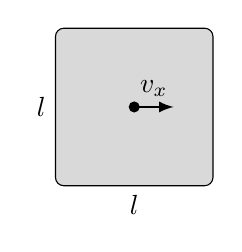
\begin{tikzpicture}
        \filldraw[color=black, fill=gray!30, rounded corners=3pt] (0, 0) rectangle (2, 2);
        \node[below] at (1, 0) {$l$};
        \node[left] at (0, 1) {$l$};
        \draw[thick, -latex] (1, 1) -- node[above] {$v_x$} ++ (0.5, 0) ;
        \fill (1, 1) circle (2pt);
    \end{tikzpicture}
    \caption{气体分子运动与压强}
\end{figure}
由于气体分子在x方向上每折返一次就会与容器壁发生一次碰撞,所以$\Delta t$时间内会与容器壁碰撞$\frac{v\Delta t}{2l}$次。因此这段时间内容器壁受到来自气体分子的冲量为
\begin{equation*}
    2mv\cdot\frac{v_x\Delta t}{2l}=\frac{m{v_x}^2}{l}\Delta t
\end{equation*}
即相当于单个气体分子给予容器壁$F=\frac{m{v_x}^2}{l}$大小的力,相对应的就会有
\begin{equation*}
    P=\frac{F}{l^2}=\frac{m{v_x}^2}{l^3}=\frac{m{v_x}^2}{V}
\end{equation*}
大小的压强。此外,该气体分子也会在y和z方向上做同样的运动,所以其速度的平均值为$\overline{v^2}=\overline{{v_x}^2}+\overline{{v_y}^2}+\overline{{v_z}^2}$。同时,容器内倘若有N个这样的气体分子,那么其压强的总和为
\begin{equation*}
    P=N\cdot\frac{m{v_x}^2}{V}=\frac{Nm\overline{v^2}}{3V}
\end{equation*}
将上述压强值代入理想气体状态方程就可以得到1摩尔该气体分子平均速度的平方。
\begin{gather*}
    PV=nRT\\
    \frac{Nm\overline{v^2}}{3V}V=\frac{N}{N_A}RT\\
    \overline{v^2}=\frac{3RT}{M}
\end{gather*}
那么n摩尔该气体分子的总动能可求。
\begin{equation*}
    n\cdot\frac12M\overline{v^2}=\frac32nRT
\end{equation*}

\subsection{等温变化做功}

\begin{equation*}
    Q_\textrm{吸}=W_\textrm{した}=\int_{V_1}^{V_2}PdV=nRT\cdot\log\frac{V_2}{V_1}
\end{equation*}

\subsection{断热变化PV等式推导}

基于断热变化的热力学第一定律可得
\begin{gather*}
    \Delta U=-W_\textrm{した}\\
    nC_v\Delta T=-PdV
\end{gather*}
简做整理后对两侧分别关于T和V积分
\begin{gather*}
    \int\frac{dT}{T}=-\frac{R}{C_v}\int\frac{dV}{V}\\
    \log T=-\frac{R}{C_v}\log V+c^\prime\\
    T=V^{-\frac{R}{C_v}}\cdot c\\
    TV^{\frac{R}{C_v}}=c
\end{gather*}
在此定义$\gamma=\frac{C_p}{C_v}$,结合$C_p-C_v=R$即有
\begin{equation*}
    TV^{\gamma-1}=c
\end{equation*}
再结合理想气体状态方程就可以得到$PV^\gamma=const$的结论。

% extra contents of chap3

\section{波动延伸}

\subsection{波的解析式推导法二}

假设$t=0$时刻的波形为
\begin{equation*}
    y_0=A\sin\left(\frac{2\pi}{\lambda}x\right)
\end{equation*}
那么$t$时间后改图像会向右平移$vt$单位长度,即
\begin{equation*}
    y=A\sin\left(\frac{2\pi}{\lambda}\left(x-vt\right)\right)
    =A\sin\left(2\pi\left(\frac{x}{\lambda}-\frac{t}{T}\right)\right)
\end{equation*}

\subsection{差频公式推导}

设两束声波分别为$y_1=\sin((\omega+\theta)t)$和$y_2=\sin((\omega-\theta)t)$,其中$\omega$远大于$\theta$。那么,根据波的叠加原理可知合成波为
\begin{align*}
    y=&\sin((\omega+\theta)t)+\sin((\omega-\theta)t)\\
    =&(\sin\omega t\cos\theta t+\cos\omega t\sin\theta t)+(\sin\omega t\cos\theta t-\cos\omega t\sin\theta t)\\
    =&(2\cos\theta t)\sin\omega t
\end{align*}
此外,声音的强度与振幅的平方相关,所以合成波的波峰与波谷都会被人耳当成差频接收。因此差频的频率为合成波括号中控制振幅部分频率的两倍。
\begin{align*}
    f=&2\times\frac{\theta}{2\pi}\\
    =&\frac{\omega_1-\omega_2}{2\pi}\\
    =&f_1-f_2
\end{align*}

\subsection{光程公式推导}

使波长为$\lambda$的波在折射率为$n$的介质中传播$l$长的距离,那么在这段空间中存在$\frac{l}{\lambda^\prime}=\frac{nl}{\lambda}$个波。倘若把这些波换算到真空中($n=1$)中,则需要
\begin{equation*}
    L=\frac{l}{\lambda^\prime}\times\lambda=nl
\end{equation*}
的距离。称$L$为光程,满足$L=nl$。

\subsection{双缝干涉光程差推导}

\begin{equation*}
    |S_1P-S_2P|=S_2H\approx d\sin\theta\approx d\tan\theta=\frac{dx}{l}
\end{equation*}

\subsection{薄膜干涉光程差推导}

根据三角关系以及折射定律可知
\begin{equation*}
    \begin{cases}
        AH=AB\sin\phi\\
        BD=AB\sin\theta\\
        \sin\theta=n\sin\phi
    \end{cases}
\end{equation*}
即$n\cdot AH=BD$,$AH$与$BD$等光程。也就是说两束光到B点前的光程差为$HC+BC$。在此,将$BC$向下对称翻转得到$BC^\prime$,因而
\begin{equation*}
    HC+BC=HC+BC^\prime=HC^\prime=2d\cos\phi
\end{equation*}
由于这个距离是折射率为$n$的介质中的,所以其真空中等效的光程为$2nd\cos\phi$。

\subsection{牛顿环干涉光程差推导}

结合勾股定理关于$R$、$r$、$d$列方程即可。
\begin{align*}
    R^2=&r^2+(R-d)^2\\
    r^2=&(2R-d)d\\
    \downarrow&\quad R\gg d\\
    r^2=&2Rd
\end{align*}

% extra contents of chap4

\section{电磁延伸}

\subsection{点电荷电势推导}

\begin{gather*}
    U=\int_r^\infty k\frac{Qq}{x^2}dx=k\frac{Qq}{r}\\
    V=\frac{U}{q}=k\frac{Q}{r}
\end{gather*}

\subsection{电容器储能公式推导}

\begin{equation*}
    U=\int_0^Q\frac{q}{C}dq=\frac{Q^2}{2C}
\end{equation*}

\subsection{电容器储能损耗推导}

假设电路中除电容器以外的外阻为$R$,则回路方程为
\begin{equation*}
    E=RI+\frac{Q}{C}\implies
    \frac{dQ}{dt}=I=\frac{E-\frac{Q}{C}}{R}
\end{equation*}
对等式两边积分可得电荷量随时间变化的函数
\begin{gather*}
    \int\frac{dQ}{E-\frac{Q}{C}}=\int\frac{dt}{R}\\
    -C\log\left\lvert E-\frac{Q}{C}\right\rvert=\frac{t}{R}+\gamma\\
    E-\frac{Q}{C}=\Gamma\exp\left(\frac{t}{RC}\right)\quad\left(\Gamma=\exp\left(-\frac{\gamma}{C}\right)\right)\\
\end{gather*}
根据初始条件$(t,Q)=(0,0)$可得$\Gamma=E$,因此
\begin{equation*}
    Q(t)=CE\left(1-\exp\left(-\frac{t}{RC}\right)\right)
\end{equation*}
最后使用$W=I^2Rt$积分求解即可
\begin{gather*}
    I=\frac{dQ}{dt}=\frac{E}{R}\exp\left(-\frac{t}{RC}\right)\\
    W=\int_0^\infty I^2Rdt=\frac12CE^2
\end{gather*}

\subsection{直线电流磁场推导}

根据Biot-Savart定律可得
\begin{align*}
    \mathbf{B}=&\frac{\mu_0}{4\pi}\int_{-\infty}^{\infty}\mathbf{J}\times\frac{\mathbf{r}-\mathbf{l}}{|\mathbf{r}-\mathbf{l}|^3}d^3l\\
    =&\frac{\mu_0I}{4\pi}\int_{-\infty}^{\infty}d\mathbf{l}\times\frac{\mathbf{r}-\mathbf{l}}{|\mathbf{r}-\mathbf{l}|^3}
\end{align*}
设$(0,0,r_z)$为矢量基准点,则可简记$r=(r_x,r_y,0)$
\begin{align*}
    \mathbf{B}=&\frac{\mu_0I}{4\pi}\int_{-\infty}^{\infty}dl\cdot e_z\times\frac{r_xe_x+r_ye_y-le_z}{|r^2+l^2|^{3/2}}\\
    =&\frac{\mu_0I}{4\pi}\int_{-\infty}^{\infty}dl\frac{r_xe_y-r_ye_x}{|r^2+l^2|^{3/2}}
\end{align*}
关于$l$求解反常积分可得
\begin{align*}
    \mathbf{B}=&\frac{\mu_0I}{4\pi}\left[\frac{l(r_xe_y-r_ye_x)}{r^2\sqrt{r^2+l^2}}\right]_{-\infty}^{\infty}\\
    =&\frac{\mu_0I}{2\pi r^2}(r_xe_y-r_ye_x)
\end{align*}
将结果改写为位置向量的形式
\begin{equation*}
    \mathbf{B}=\frac{\mu_0I}{2\pi r^2}(-r_y,r_x,0)
\end{equation*}
即大小为$B=\frac{\mu_0I}{2\pi r}$,方向与$\mathbf{r}$垂直的磁场。

另外,倘若使用Ampère's circuital law则可以更加方便地求解。
\begin{align*}
    \oint_{\partial S}B\cdot dl=&\mu_0I\\
    2\pi r B=&\mu_0I\\
    B=&\frac{\mu_0I}{2\pi r}
\end{align*}

\subsection{环形电流磁场推导}

设位于xy平面上的环形电流半径为$r$,计算z轴上点$\mathbf{z}=(0,0,z)$处的磁场。则根据Biot-Savart定律$\mathbf{l}=(l\cos\phi,l\sin\phi,0)$处的微小电流产生的磁场即为
\begin{align*}
    d\mathbf{B}=&\frac{\mu_0I}{4\pi}\frac{d\mathbf{l}\times(\mathbf{z}-\mathbf{l})}{|\mathbf{z}-\mathbf{l}|^3}\\
    =&\frac{\mu_0I}{4\pi|\mathbf{z}-\mathbf{l}|^3}(-\sin\phi,\cos\phi,0)dl\times(-l\cos\phi,-l\sin\phi,r)\\
    =&\frac{\mu_0I}{4\pi|\mathbf{z}-\mathbf{l}|^3}(r\cos\phi,r\sin\phi,l)dl
\end{align*}
分别关于xyz三个方向积分可得
\begin{align*}
    \begin{cases}
        B_x=\frac{\mu_0}{4\pi}\oint\frac{z\cos\phi}{|\mathbf{z}-\mathbf{l}|^3}dl
        =\frac{\mu_0}{4\pi}\int_0^{2\pi}\frac{z\cos\phi}{|\mathbf{z}-\mathbf{l}|^3}ld\phi=0\\
        B_y=\frac{\mu_0}{4\pi}\oint\frac{z\sin\phi}{|\mathbf{z}-\mathbf{l}|^3}dl=0\\
        B_z=\frac{\mu_0}{4\pi}\oint\frac{l}{|\mathbf{z}-\mathbf{l}|^3}dl
        =\frac{\mu_0}{4\pi}\oint\frac{ldl}{(z^2+l^2)^{3/2}}=\frac{\mu_0Il^2}{2(z^2+l^2)^{3/2}}\\
    \end{cases}
\end{align*}
可见除$B_z$以外的磁场均为0,并且当$z=0$时$B_z=\frac{\mu_0I}{2l}$的确成立。

\subsection{线圈磁场推导}

\begin{figure}[ht!]
    \centering
    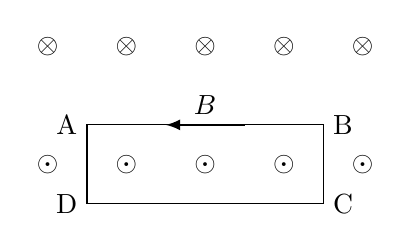
\begin{tikzpicture}
        \foreach \x in {0,...,4} {
            \node at (\x, 0) {$\odot$};
            \node at (\x, 1.5) {$\otimes$};
        }
        \draw (0.5,-0.5) -- (0.5,0.5) node[left] {A} -- (3.5,0.5) node[right] {B} -- (3.5,-0.5) node[right] {C} -- (0.5,-0.5) node[left] {D} --cycle;
        \draw[thick, -latex] (2.5,0.5) -- node[above] {$B$} (1.5,0.5);
    \end{tikzpicture}
    \caption{线圈磁场截面}
\end{figure}
如图所示,确定一个固定路径,采用Ampère's circuital law进行计算。
\begin{gather*}
    \oint_{\partial S}B\cdot dl=\mu_0\int_Sj\cdot dS\\
    \underline{Bl}_{AB}+\underline{0}_{BC}+\underline{0}_{CD}+\underline{0}_{DA}=\mu_0I\cdot nl\\
    B=\mu_0nI
\end{gather*}

\subsection{洛伦兹力推导}

使用电流的微观定义计算单个载流子的受力即可。
\begin{equation*}
    \vec{f}=\frac{\vec{F}}{N}=\frac{I\vec{l}\times\vec{B}}{N}
    =\frac{nqSl\vec{v}\times\vec{B}}{nSl}
    =q\vec{v}\times\vec{B}
\end{equation*}

\subsection{带电粒子在磁场中运动轨迹推导}

在静磁场中带电粒子的运动方程为
\begin{equation*}
    m\frac{d^2\mathbf{r}}{dt^2}=q\frac{d\mathbf{r}}{dt}\times\mathbf{B}
\end{equation*}
假设该静磁场只存在于z方向,即$\mathbf{B}=(0,0,B)$
\begin{equation*}
    m\begin{pmatrix}
     \ddot{x}\\\ddot{y}\\\ddot{z}   
    \end{pmatrix}=
    q\begin{pmatrix}
        \dot{x}\\\dot{y}\\\dot{z}
    \end{pmatrix}\times
    \begin{pmatrix}
        0\\0\\B
    \end{pmatrix}=
    qB\begin{pmatrix}
        \dot{y}\\-\dot{x}\\0
    \end{pmatrix}
\end{equation*}
其中z方向的运动方程为$m\ddot{z}=0$,即粒子在z方向做匀速直线运动。而后,使用极坐标系处理xy平面的运动,基于其转换关系
\begin{itemize}
    \item 速度:$\begin{cases}v_r=\dot{r}\\v_\phi=r\dot{\phi}\end{cases}$
    \item 加速度:$\begin{cases}a_r=\ddot{r}-r\dot{\phi}^2\\a_\phi=2\dot{r}\dot{\phi}+r\ddot{\phi}\end{cases}$
\end{itemize}
即
\begin{align*}
    \begin{cases}
        a_r=a_x\cos\phi+a_y\sin\phi
        =\frac{qB}{m}\left(v_y\cos\phi-v_x\sin\phi\right)
        =\frac{qB}{m}v_\phi\\
        a_\phi=-a_x\sin\phi+a_y\cos\phi
        =-\frac{qB}{m}\left(-v_y\sin\phi+v_x\cos\phi\right)
        =-\frac{qB}{m}v_r\\
    \end{cases}
\end{align*}
代入运动方程可得
\begin{equation*}
    \begin{cases}
        \ddot{r}-r\dot{\phi}^2=\frac{qB}{m}r\dot{\phi}\\
        2\dot{r}\dot{\phi}+r\ddot{\phi}=-\frac{qB}{m}\dot{r}
    \end{cases}
    \implies
    \begin{cases}
        \frac{\ddot{r}}{r}=\dot{\phi}\left(\frac{qB}{m}+\dot{\phi}\right)\\
        \ddot{\phi}=-\frac{\dot{r}}{r}\left(\frac{qB}{m}+2\dot{\phi}\right)
    \end{cases}
\end{equation*}
其中一式左右两边变量完全独立,因此可以拆成两个分别等于零的式子
\begin{equation*}
    \begin{cases}
        \frac{\ddot{r}}{r}=0\\
        \dot{\phi}\left(\frac{qB}{m}+\dot{\phi}\right)=0\\
        \ddot{\phi}=-\frac{\dot{r}}{r}\left(\frac{qB}{m}+2\dot{\phi}\right)
    \end{cases}
\end{equation*}
求解联立微分方程组可得
\begin{equation*}
    \begin{cases}
        \ddot{r}=0\\
        \dot{\phi}=-\frac{qB}{m}\\
        \dot{r}=0
    \end{cases}
\end{equation*}
其物理意义即为粒子在r方向上不受力、在$\phi$方向上保持恒定角速度$\frac{qB}{m}$做圆周运动。再结合z方向的匀速直线运动可知,粒子在空间上的轨迹为圆柱螺线。

\subsection{含自感直流电路的电流表达式推导}

结合自感电势和基尔霍夫定律可得
\begin{equation*}
    E-IR+V=0
\end{equation*}
即
\begin{equation*}
    \frac{dI}{dt}=\frac{E-IR}{L}
\end{equation*}
此微分方程可解
\begin{equation*}
    I=\frac{E}{R}\left(1+C\exp\left(-\frac{R}{L}t\right)\right)
\end{equation*}
在初始条件$(t,I)=(0,0)$下可知
\begin{equation*}
    I=\frac{E}{R}\left(1-\exp\left(-\frac{R}{L}t\right)\right)
\end{equation*}

\subsection{自感线圈储能公式推导}

\begin{equation*}
    U=W=qV
    =\int_0^I(Idt)\left(L\frac{dI}{dt}\right)
    =\frac12LI^2
\end{equation*}

\subsection{交流电平均电功率推导}

\begin{equation*}
    P=\frac{W}{T}
    =\frac1T\int_0^TI_0V_0\sin^2\omega tdt
    =\frac12I_0V_0
\end{equation*}

\subsection{交流电电容器结论推导}

\paragraph{电流} $I=\frac{dQ}{dt}=\frac{d(CV_0\sin\omega t)}{dt}=\omega CV_0\cos\omega t$

\paragraph{平均功率} $\bar{P}=IV=\frac1T\int_0^TI_0V_0\cos\omega t\sin\omega tdt=0$

\subsection{交流电线圈结论推导}

\paragraph{电流} 根据自感线圈电压表达式以及基尔霍夫定律可得
\begin{equation*}
    V_0\sin\omega t-L\frac{dI}{dt}=0
\end{equation*}
整理后可得
\begin{equation*}
    dI=\frac{V_0}{L}\sin\omega tdt
\end{equation*}
即
\begin{equation*}
    I=-\frac{V_0}{\omega L}\cos\omega t
\end{equation*}

\paragraph{平均功率} $\bar{P}=IV=-\frac1T\int_0^TI_0V_0\cos\omega t\sin\omega tdt=0$


\chapter{真题略解}

部分真题可参见EJU官网\footnote{\url{https://www.jasso.go.jp/ryugaku/eju/examinee/pastpaper_sample/index.html}}。

% brief answers of 15h27a

\section{15年第一回(H27A)}

\paragraph{1. (\hyperref[subsec:1.1.3]{1.1.3})}

\begin{equation*}
    m_1g(l\cos\theta-d\sin\theta)=m_2g(l\cos\theta+d\sin\theta)
\end{equation*}

\paragraph{2. (\hyperref[subsec:1.1.2]{1.1.2})} 弹性碰撞,无能量损失,可考虑对称展开。

\begin{equation*}
    \begin{cases}
        h=\frac12gt^2\\
        2L=vt
    \end{cases}
\end{equation*}

\paragraph{3. (\hyperref[subsec:1.2.2]{1.2.2})}

\begin{gather*}
    v_A'=\frac{m_Av_A-em_Bv_A}{m_A+m_B}=\frac{m_A-m_B}{m_A+m_B}v\\
    I=m_A(v_A'-v_A)=-\frac{2m_Am_B}{m_A+m_B}v
\end{gather*}

\paragraph{4. (\hyperref[subsec:1.2.1]{1.2.1})}

\begin{gather*}
    mg=kv\\
    P=Fv=mg\times\frac{mg}{k}=\frac{(mg)^2}{k}
\end{gather*}

\paragraph{5. (\hyperref[subsec:1.2.2]{1.2.2})}

\begin{equation*}
        W=E_k=\frac{mv^2}{2}=\frac{p^2}{2m}\\
\end{equation*}

\paragraph{6. (\hyperref[subsec:1.3.1]{1.3.1})}

\begin{gather*}
    F_\textrm{向}=T+G\\
    T=m\frac{v^2}{r}-mg
\end{gather*}

\paragraph{7. (\hyperref[sec:2.1]{2.1})}

\begin{gather*}
    Q_\textrm{总}=10\times50\times60=3\times10^4J\\
    Q_\textrm{冰升温}=2.1\times100\times20=4.2\times10^3J\\
    Q_\textrm{冰融化}=330\times100=3.3\times10^4J\\
    \therefore\textrm{冰无法全部融化成水}
\end{gather*}

\paragraph{8. (\hyperref[subsec:2.2.2]{2.2.2})} 从效果考虑对外做功的大小。

\begin{gather*}
    \Delta U=Q_\textrm{吸}+W_\textrm{された}\\
    Q_\textrm{吸}=\Delta U+W_\textrm{した}\\
    \begin{cases}
        \Delta U=\frac32nR\Delta T=nC_v\Delta T\\
        W_\textrm{した}=p_0S\Delta x+\frac12k\Delta x^2
    \end{cases}
\end{gather*}

\paragraph{9. (\hyperref[subsec:2.2.3]{2.2.3})}

\begin{gather*}
    \begin{array}{c|ccc}
        & \Delta U & Q_\textrm{吸} & W_\textrm{された} \\\hline
        A\to B & - & - & 0 \\
        B\to C & 0 & - & + \\
        C\to A & + & + & - \\
    \end{array}\\
    \eta=\frac{W_\textrm{对外实际做功}}{Q_\textrm{纯吸热}}
    =\frac{\frac12\times\frac14p_0\times\frac14v_0}{\frac32\times p_0\times\frac14v_0+p_0\times\frac14v_0}=\frac{1}{20}
\end{gather*}

\paragraph{10. (\hyperref[subsec:3.1.1]{3.1.1})} 略
\paragraph{11. (\hyperref[subsec:3.1.2]{3.1.2})} 需注意此时缝间距并不远小于A到B的距离,因此不应使用双缝干涉公式。

\begin{equation*}
    |r_1-r_2|=1=2m\times\frac\lambda2\quad(m=2)\\
\end{equation*}

\paragraph{12. (\hyperref[subsec:3.3.1]{3.3.1})}

\begin{equation*}
    \frac1a+\frac1b=\frac1f\implies
    \begin{cases}
        |b|=\left|\frac{af}{a-f}\right|=\frac{f}{f/a-1}\\
        m=\left|\frac{b}{a}\right|=\left|\frac{f}{a-f}\right|
    \end{cases}
\end{equation*}

\paragraph{13. (\hyperref[subsec:4.1.1]{4.1.1})} 略
\paragraph{14. (\hyperref[subsec:4.1.3]{4.1.3})} BC连通后等电势,相当于BC间被抽出,后用平行板电容器电容量定义是计算即可。

\paragraph{15. (\hyperref[subsec:4.2.2]{4.2.2})} 设左右两部分均为顺时针电流,记作$I_1$和$I_2$,并设AB段为$I_1-I_2$。

\begin{equation*}
    \begin{cases}
        \textrm{左}: 6-10I_1-10(I_1-I_2)=0\\
        \textrm{右}: 6+10(I_1-I_2)-10I_2=0
    \end{cases}\implies
    I_1-I_2=0
\end{equation*}

\paragraph{16. (\hyperref[subsec:4.3.1]{4.3.1})}

\begin{equation*}
    \begin{cases}
        \textrm{图1}: \vec{H}=(0,0,H)\\
        \textrm{图2}: \vec{H}=0\implies \vec{H_{2//x}}=(0,0,-H)\\
        \textrm{图3}: \vec{H}=\vec{H_1}+\vec{H_{2//z}}=(0,0,H)+(H,0,0)
    \end{cases}
\end{equation*}

\paragraph{17. (\hyperref[subsec:4.3.2]{4.3.2})} 略
\paragraph{18. (\hyperref[subsec:4.4.1]{4.4.1})} 略
\paragraph{19. (\hyperref[sec:5.2]{5.2})}

\begin{equation*}
    \frac{\frac{mv^2}{r}}{mvr}=\frac{\frac{ke^2}{r^2}}{\frac{nh}{2\pi}}\implies
    v=\frac{2\pi ke^2}{nh}
\end{equation*}

% brief answers of 15h27b

\section{15年第二回(H27B)}

\paragraph{1. (\hyperref[subsec:1.1.3]{1.1.3})}

\begin{equation*}
    2G\times L\cos\theta=G\times\frac{L}{2}\sin\theta
\end{equation*}

\paragraph{2. (\hyperref[subsec:1.1.1]{1.1.1})}

\begin{equation*}
    \begin{cases}
        v^2=2ax\\
        v=at
    \end{cases}\implies
    v=\frac{2x}{t}
\end{equation*}

\paragraph{3. (\hyperref[subsec:1.1.2]{1.1.2})} 旋转视角至BC水平,则该物体同时具有向下和向右的加速度,且大小均为$g'=\frac{g}{\sqrt{2}}$。

\begin{equation*}
    \begin{cases}
        t=\frac{2v}{g'}\\
        \sqrt{2}h=\frac12g't^2
    \end{cases}
\end{equation*}

\paragraph{4. (\hyperref[subsec:1.2.1]{1.2.1})} 一般能量解法优于运动解法。

\subparagraph{能量解法} 以出发点为重力势能基准。

\begin{equation*}
    \begin{cases}
        mg=kd\\
        \frac12k(3d)^2=\frac12mv^2+3mgd
    \end{cases}\implies
    v=\sqrt{3gd}
\end{equation*}

\subparagraph{运动解法}

\begin{gather*}
    x=A\cos\omega t=2d\cos\sqrt{\frac{k}{m}}t\\
    v=\frac{dx}{dt}=-2d\sqrt{\frac{k}{m}}\sin\sqrt{\frac{k}{m}}t\\
    x=-d\implies t=\sqrt{\frac{k}{m}}\times\frac23\pi\ or\ \sqrt{\frac{k}{m}}\times\frac43\pi\\
    |v|=\left|-2d\sqrt{\frac{k}{m}}\sin\left(\frac23\pi\ or\ \frac43\pi\right)\right|=\sqrt{\frac{3k}{m}}d\\
    mg=kd\implies|v|=\sqrt{3gd}
\end{gather*}

\paragraph{5. (\hyperref[subsec:1.2.2]{1.2.2})} 基于A与B无相对运动和动量守恒可解。
\paragraph{6. (\hyperref[subsec:1.3.1]{1.3.1})}

\begin{gather*}
    \begin{cases}
        F_\textrm{向}=mg\sin30^\circ\\
        \frac12mv_0^2=\frac12mv^2+mgr(1+\sin30^\circ)
    \end{cases}
\end{gather*}

\paragraph{7. (\hyperref[sec:2.1]{2.1})}

\begin{gather*}
    \begin{cases}
        c_A\times0.1\times15=3000\\
        c_B\times0.1\times10=4000
    \end{cases}\implies
    \begin{cases}
        c_A=2000\\
        c_B=4000
    \end{cases}\\
    2000\times0.4\times t+4000\times0.3\times t=10000
\end{gather*}

\paragraph{8. (\hyperref[subsec:2.2.2]{2.2.2})}

\begin{gather*}
    \begin{cases}
        pV_A=n_ART\\
        pV_B=n_BRT
    \end{cases}\implies
    \frac{V_A}{V_B}=\frac{n_A}{n_B}=\frac{N_A}{N_B}
\end{gather*}
\begin{equation*}
    \frac12m\overline{v^2}\times N=\frac32nRT\implies
    \overline{v^2}\propto\frac1m
\end{equation*}

\paragraph{9. (\hyperref[subsec:2.2.2]{2.2.2})}

\begin{gather*}
    \begin{array}{c|ccc}
        & \Delta U & Q_\textrm{吸} & W_\textrm{された} \\\hline
        A\to B & - & - & 0 \\
        B\to C & + & + & -
    \end{array}\\
    Q_\textrm{实际吸热}=n(C_p-C_v)T_0=nRT_0
\end{gather*}

\paragraph{10. (\hyperref[subsec:3.1.3]{3.1.3})} 需区分波面和波的传播方向。
\paragraph{11. (\hyperref[subsec:3.1.2]{3.1.2})}

\begin{align*}
    |r_1-r_2|=&(2m-1)\frac\lambda2\\
    1=&\lambda\left(m-\frac12\right)\\
    f=&v\left(m-\frac12\right),\quad f\ge500Hz\\
    f=&510Hz,\quad m=2
\end{align*}

\paragraph{12. (\hyperref[subsec:3.3.2]{3.3.2})}

\begin{gather*}
    a=\Delta x=\frac{\lambda l}{d}\implies
    \frac{a'}{a}=\frac{d}{d'}=\frac23
\end{gather*}

\paragraph{13. (\hyperref[subsec:4.1.2]{4.1.2})}

\begin{gather*}
    \begin{cases}
        V_D=\frac{kq}{a}-\frac{8kq}{2a}=-\frac{3kq}{a}\\
        V_C=\frac{kq}{2a}-\frac{8kq}{a}=-\frac{15kq}{2a}
    \end{cases}\implies
    V_D-V_C=\frac{9kq}{2a}
\end{gather*}

\paragraph{14. (\hyperref[subsec:4.1.3]{4.1.3})} 串联电荷相等。

\begin{equation*}
    E=\frac{V}{d}=\frac{Q}{Cd}\xRightarrow[d_A=d_B]{Q_A=Q_B}
    \frac{E_B}{E_A}=\frac{C_A}{C_B}=\frac{C}{\epsilon C}=\frac1\epsilon
\end{equation*}

\paragraph{15. (\hyperref[subsec:4.2.1]{4.2.1})} 略
\paragraph{16. (\hyperref[subsec:4.3.1]{4.3.1})} 略
\paragraph{17. (\hyperref[subsec:4.3.2]{4.3.2})} 左手定则判断并做力的合成即可。
\paragraph{18. (\hyperref[subsec:4.4.1]{4.4.1})} 楞次定律判断并将导体棒视作电源即可。
\paragraph{19. (\hyperref[sec:5.2]{5.2})}

\begin{gather*}
    E_4-E_2=\frac{hc}{\lambda}\\
    \lambda=\frac{hc}{E_4-E_2}
    =\frac{6.6\times10^{-34}\times3\times10^8}{\frac{-2.2\times10^{-18}}{16}-\frac{-2.2\times10^{-18}}{4}}
    =4.8\times10^{-7}
\end{gather*}

% brief answers of 16h28a

\section{16年第一回(H28A)}

\paragraph{1. (\hyperref[subsec:运动与力]{运动与力})} 受力分析,观察二次导数值即可。

\begin{gather*}
    F-mg=ma\\
    F=mg+\frac{d^2}{dt^2}h
\end{gather*}

\paragraph{2. (\hyperref[subsec:运动与力]{运动与力})}

\begin{equation*}
    \frac{F}{m+M}=\frac{\mu mg}{M}
\end{equation*}

\paragraph{3. (\hyperref[subsec:能量]{能量}, \hyperref[subsec:动量]{动量})}

\begin{equation*}
    \frac12mv^2=mgH\implies
    H=\frac{v^2}{2g}
\end{equation*}

\begin{gather*}
    mv=(m+M)v'\\
    v'=\frac{m}{m+M}v\\
    \frac12mv^2=mgh+\frac12(m+M)\left(\frac{m}{m+M}v\right)^2\\
    h=\frac{M}{m+M}\frac{v^2}{2g}
\end{gather*}

\paragraph{4. (\hyperref[subsec:动量]{动量})} F-t图像中面积为冲量。
\paragraph{5. (\hyperref[subsec:运动与力]{运动与力}, \hyperref[subsec:简谐振动]{简谐振动})} 略
\paragraph{6. (\hyperref[subsec:圆周运动]{圆周运动})}

\begin{equation*}
    \begin{cases}
        F_\textrm{向}=mg\cos\theta\\
        \frac12mv^2=mgr(1-\cos\theta)+\frac12mv_0^2
    \end{cases}
\end{equation*}

\paragraph{7. (\hyperref[sec:热与能量]{热与能量})}

\begin{gather*}
    2\times10^3\times1\times(10\Delta t)+1\times10^3\times(10\Delta t)=P\times\Delta t\\
    P=3\times10^4\\
    3.3\times10^5\times1=P\times t\\
    t=11
\end{gather*}

\paragraph{8. (\hyperref[subsec:气体法则]{气体法则})}

\begin{gather*}
    \begin{cases}
        A: 8p\cdot V=n_ART\\
        B: p\cdot 4V=n_BRT
    \end{cases}\\
    n_A'=\frac{V}{V+4V}(n_A+n_B)
\end{gather*}

\paragraph{9. (\hyperref[subsec:气体状态变化]{气体状态变化})} 略
\paragraph{10. (\hyperref[subsec:衍射·反射·折射]{衍射·反射·折射})} 略
\paragraph{11. (\hyperref[subsec:多普勒效应]{多普勒效应})} 平面多普勒效应,从圆上优劣弧着手,分析最值变化即可。
\paragraph{12. (\hyperref[subsec:光的干涉]{光的干涉})}

\begin{gather*}
    2x\tan\theta=m\lambda\\
    \Delta x=\frac{\lambda}{2\tan\theta}=\frac{\lambda L}{2D}
\end{gather*}

\paragraph{13. (\hyperref[subsec:电场]{电场})} 略
\paragraph{14. (\hyperref[subsec:电势]{电势})} 略
\paragraph{15. (\hyperref[subsec:欧姆定律]{欧姆定律})} 根据电阻定义式可知$R_Y=2R_X$,后根据电功率公式$P=\frac{V^2}{R}$计算即可。
\paragraph{16. (\hyperref[subsec:电容器]{电容器})} 可按照电容器并联处理电荷分配。

\begin{gather*}
    V'=\frac{Q_A}{C_A+C_B}\\
    U_A=U_A'+U_B'+W_R\\
    W_R=\frac12C_AV^2-\frac12(C_A+C_B)V'^2
\end{gather*}

\paragraph{17. (\hyperref[subsec:磁场]{磁场})} 略
\paragraph{18. (\hyperref[subsec:洛伦兹力]{洛伦兹力})}

\begin{gather*}
    qV=\frac12mv^2\implies v=\sqrt{\frac{2qV}{m}}\\
    r=\frac{mv}{qB}=\frac1B\sqrt{\frac{2mV}{q}}\\
    \frac{m'}{m}=\left(\frac{r'}{r}\right)^2=16
\end{gather*}

\paragraph{19. (\hyperref[sec:波粒二象性]{波粒二象性})} 略

% brief answers of 16h28b

\section{16年第二回(H28B)}

\paragraph{1. (\hyperref[subsec:1.1.2]{1.1.2})} 略
\paragraph{2. (\hyperref[subsec:1.1.1]{1.1.1})} v-t图像中面积为路程。
\paragraph{3. (\hyperref[subsec:1.1.2]{1.1.2})}

\begin{gather*}
    \frac12m(v_0\sin\theta)^2=mgH\\
    H=\frac{(v_0\sin\theta)^2}{2g}\\
    t=2\times\frac{v_0\sin\theta}{g}\\
    L=v_0\sin\theta\times t=\frac{2v_0^2\sin\theta\cos\theta}{g}
\end{gather*}

\paragraph{4. (\hyperref[subsec:1.2.1]{1.2.1}, \hyperref[subsec:1.2.2]{1.2.2})} 略
\paragraph{5. (\hyperref[subsec:1.2.2]{1.2.2})}

\begin{equation*}
    \begin{cases}
        mv_0=2mv_B\cos\theta+mv_A\cos\theta\\
        2mv_B\sin\theta=mv_A\sin\theta
    \end{cases}
\end{equation*}

\paragraph{6. (\hyperref[subsec:1.3.1]{1.3.1})}

\begin{equation*}
    \begin{cases}
        mgl\cos\theta=\frac12mv^2\\
        T-mg\cos\theta=\frac{mv^2}{l}
    \end{cases}
\end{equation*}

\paragraph{7. (\hyperref[sec:2.1]{2.1})}

\begin{gather*}
    2.1\times20\times20+20\times330+4.2\times20\times T=4.2\times100\times(20-T)\\
    T\approx 1.9
\end{gather*}

\paragraph{8. (\hyperref[subsec:2.2.2]{2.2.2})}

\begin{gather*}
    \begin{cases}
        1\times10^5\times6\times10^{-3}=nR\cdot300\\
        1\times10^5\times V=nR\cdot 400
    \end{cases}\\
    W=p\Delta V=1\times10^5\times(8\times10^{-3}-6\times10^{-3})=200J
\end{gather*}

\paragraph{9. (\hyperref[subsec:2.2.3]{2.2.3})} 略
\paragraph{10. (\hyperref[subsec:3.1.1]{3.1.1})} 略
\paragraph{11. (\hyperref[subsec:3.2.2]{3.2.2})}

\begin{gather*}
    f_A<f_b\implies f_B=f_A+n\\
    \frac{V+u}{V}f=\frac{V-u}{V}(f+n)\\
    \frac{u}{V}=\frac{n}{n+2f}
\end{gather*}

\paragraph{12. (\hyperref[subsec:3.3.1]{3.3.1})} 略
\paragraph{13. (\hyperref[subsec:4.1.1]{4.1.1})} 略
\paragraph{14. (\hyperref[subsec:4.1.2]{4.1.2})}

\begin{align*}
    W=&W_{A\to O}-W_{B\to O}\\
    =&U_A-U_B\\
    =&-2q\left(\frac{kq}{d}-\frac{kq}{5d}\right)\\
    =&-\frac85\frac{kq^2}{d}
\end{align*}

\paragraph{15. (\hyperref[subsec:4.1.3]{4.1.3})}

\begin{gather*}
    Q_P=V_1C\\
    (V-0)C-(V_2-V)C=Q_P\\
    2VC-V_2C=V_1C\\
    V=\frac12(V_1+V_2)
\end{gather*}

\paragraph{16. (\hyperref[subsec:4.2.2]{4.2.2})} 略
\paragraph{17. (\hyperref[subsec:4.2.2]{4.2.2})} 略
\paragraph{18. (\hyperref[subsec:4.3.2]{4.3.2})}

\begin{equation*}
    F_x=\frac{\mu I}{2\pi\sqrt{a^2+x^2}}\times I\times l\times\frac{-x}{\sqrt{a^2+x^2}}=\frac{\mu I^2l}{2\pi}\frac{-x}{a^2+x^2}
\end{equation*}

\paragraph{19. (\hyperref[sec:5.2]{5.2})}

\begin{equation*}
    T=10\times7\times10^8=7\times10^9
\end{equation*}

% brief answers of 17h29a

\section{17年第一回(H29A)}

\paragraph{1. (\hyperref[subsec:1.1.2]{1.1.2})} 略
\paragraph{2. (\hyperref[subsec:1.1.2]{1.1.2})}

\begin{equation*}
    F_0=10+f_{A+B}=10+0.5\times(6+4)\times10=60N
\end{equation*}

\paragraph{3. (\hyperref[subsec:1.2.2]{1.2.2})}

\begin{gather*}
    \begin{cases}
        x=vt\\h=\frac12gt^2
    \end{cases}\implies
    \frac{x_B}{x_A}=\frac{v_B}{v_A}
    \xlongequal{\begin{cases}
        v_A=\frac{mv-emv}{2m}\\
        v_B=\frac{mv+emv}{2m}
    \end{cases}}
    \frac{1+0.6}{1-0.6}=4
\end{gather*}

\paragraph{4. (\hyperref[subsec:1.3.1]{1.3.1})}

\begin{equation*}
    \begin{cases}
        T-G=F_\textrm{向}\\
        mgl+\frac12mv_0^2=\frac12mv^2
    \end{cases}
\end{equation*}

\paragraph{5. (\hyperref[subsec:1.2.1]{1.2.1}, \hyperref[subsec:1.2.2]{1.2.2})}

\begin{gather*}
    E_k=\frac{p^2}{2m}\xLongrightarrow{p_A=p_B}
    \frac{E_{kA}}{E_{kB}}=\frac{m_B}{m_A}\\
    E_p=E_{kA}+E_{kB}\\
    E_{kA}=E_p\times\frac{m_B}{m_A+m_B}
\end{gather*}

\paragraph{6. (\hyperref[subsec:1.3.3]{1.3.3})}

\begin{gather*}
    \begin{cases}
        K=\frac12mv^2\\
        G\frac{Mm}{r^2}=\frac{mv^2}{r}
    \end{cases}\implies
    K=\frac{GMm}{2r}\\
    \frac{K_B}{K_A}=\frac{\frac{m_B}{r_B}}{\frac{m_A}{r_A}}=\frac14
\end{gather*}

\paragraph{7. (\hyperref[sec:2.1]{2.1})}

\begin{gather*}
    4.2\times200\times(20-0)=2.1\times100\times(0-(-10))+330\times(100-m)\\
    330\times(100-m)=2.1\times100\times70\\
    m\approx55.4g
\end{gather*}

\paragraph{8. (\hyperref[subsec:2.2.1]{2.2.1})}

\begin{align*}
    \Delta U=&Q_\textrm{吸}+W_\textrm{された}\\
    =&2.5\times10^3-(1\times10^{-1}\times10^5)\times10^{-1}\\
    =&1.5\times10^3J
\end{align*}

\paragraph{9. (\hyperref[subsec:2.2.2]{2.2.2})}

\begin{gather*}
    \Delta U=\frac32\Delta(pV)=\frac32(6p_0V_0-p_0V_0)=\frac{15}{2}p_0V_0\\
    W_\textrm{した}=\frac12\cdot(p_0+2p_0)\cdot2V_0=3p_0V_0\\
    Q_\textrm{吸}=\Delta U+W_\textrm{した}=\frac{21}{2}p_0V_0
\end{gather*}

\paragraph{10. (\hyperref[subsec:1.3.1]{3.1.1})} 构建密度变化和纵波疏密部之间的关联即可。
\paragraph{11. (\hyperref[subsec:3.2.3]{3.2.3})}

\begin{gather*}
    l=\frac{n\lambda}{2}
    \xLongrightarrow[\lambda f=v]{v=k\sqrt{mg}}
    m=\frac{4f^2l^2}{gk^2}\times\frac{1}{n^2}\\
    \frac{m'}{m}=\left(\frac{1}{\frac12}\right)^2=4
\end{gather*}

\paragraph{12. (\hyperref[subsec:3.1.3]{3.1.3})} 略
\paragraph{13. (\hyperref[subsec:4.1.1]{4.1.1})} 略
\paragraph{14. (\hyperref[subsec:4.1.3]{4.1.3})}

\begin{equation*}
    C'=C_\textrm{左}+C_\textrm{右}
    =\varepsilon\frac{\frac23S}{d}+\varepsilon\frac{\frac13S}{\frac12d}
    =\frac43\cdot\varepsilon\frac Sd
    =\frac43C
\end{equation*}

\paragraph{15. (\hyperref[subsec:4.2.2]{4.2.2})}

\begin{equation*}
    \left(\frac{6}{1+R}\right)^2\times R=5
\end{equation*}

\paragraph{16. (\hyperref[subsec:4.3.1]{4.3.1})} 略
\paragraph{17. (\hyperref[subsec:4.3.2]{4.3.2})} 偶力为作用线平行、大小相等的一对力,其力矩可由力的大小和两个力的垂直距离的乘积计算。
\paragraph{18. (\hyperref[subsec:4.4.1]{4.4.1})} 略
\paragraph{19. (\hyperref[sec:5.2]{5.2})}

\begin{equation*}
    \frac{113-101}{2}=6
\end{equation*}

% brief answers of 17h29b

\section{17年第二回(H29B)}

\paragraph{1. (\hyperref[subsec:1.1.2]{1.1.2})} 略
\paragraph{2. (\hyperref[subsec:1.1.2]{1.1.2})}

\begin{equation*}
    F_0+\mu mg\cos\theta=mg\sin\theta
\end{equation*}

\paragraph{3. (\hyperref[subsec:1.2.1]{1.2.1})}

\begin{equation*}
    v^2=2\cdot\frac{g}{3}\cdot h
\end{equation*}

\subparagraph{整体法}

\begin{equation*}
    a=a_A=a_B=\frac{2mg-mg}{2m+m}=\frac{g}{3}
\end{equation*}

\subparagraph{隔离法}

\begin{equation*}
    \begin{cases}
        A: T-mg=mg\\
        B: 2mg-T=2ma
    \end{cases}\implies
    a=\frac{g}{3}
\end{equation*}

\paragraph{4. (\hyperref[subsec:1.2.1]{1.2.1}, \hyperref[subsec:1.2.2]{1.2.2})}

\begin{gather*}
    p_A=p_B\implies
    \begin{cases}
        \frac{v_A}{v_B}=\frac{m_B}{m_A}\\
        \frac{K_A}{K_B}\xlongequal{K=p^2/2m}\frac{m_B}{m_A}
    \end{cases}
\end{gather*}

\paragraph{5. (\hyperref[subsec:1.2.1]{1.2.1})} 一般能量解法优于运动解法。

\subparagraph{能量解法}

\begin{equation*}
    \begin{cases}
        \frac12kd^2=\frac12mv_0^2\\
        \frac12kd^2-\frac12kx^2=\frac12m\left(\frac{v_0}{2}\right)^2
    \end{cases}\implies
    \frac{d^2}{d^2-x^2}=4
\end{equation*}

\subparagraph{运动解法}

\begin{gather*}
    \begin{cases}
        x=d\cos\left(\sqrt{\frac{k}{m}}t\right)\\
        v=-d\sqrt{\frac{k}{m}}\sin\left(\sqrt{\frac{k}{m}}t\right)
    \end{cases}\implies
    x(v)=\sqrt{d^2-\frac{mv^2}{k}}\\
    x(v_0)=0\implies \frac{mv_0^2}{k}=d^2\\
    x\left(\frac{v_0}{2}\right)=\frac{\sqrt{3}}{2}d
\end{gather*}

\paragraph{6. (\hyperref[subsec:1.3.3]{1.3.3})}

\begin{equation*}
    \frac12rv_0=\frac12\cdot5r\cdot\sin\theta\quad\left(\sin\theta=\frac35\right)
\end{equation*}

\paragraph{7. (\hyperref[sec:2.1]{2.1})}

\begin{gather*}
    4.2\times1000\times(30-t)=330\times200+4.2\times200\times t\\
    t=\frac{250}{21}\approx11.9
\end{gather*}

\paragraph{8. (\hyperref[subsec:2.2.1]{2.2.1})}

\begin{gather*}
    \begin{cases}
        p_1\cdot s\cdot l_A=0.2\cdot RT\\
        p_1\cdot s\cdot l_B=0.6\cdot RT
    \end{cases}\implies l_B=3l_A\\
    \begin{cases}
        p_2\cdot s\cdot 1.5l_A=0.2\cdot RT_A\\
        p_2\cdot s\cdot (l_B-0.5l_A)=0.6\cdot RT_B
    \end{cases}\\
    \frac{T_A}{T_B}=3\cdot\frac{1.5l_A}{l_B-0.5l_A}=\frac95
\end{gather*}

\paragraph{9. (\hyperref[subsec:2.2.3]{2.2.3})} 略
\paragraph{10. (\hyperref[subsec:3.1.1]{3.1.1})} 根据y-t图像和v-t图像寻找对应特征即可。
\paragraph{11. (\hyperref[subsec:3.2.2]{3.2.2})}

\subparagraph{step1 (发射)}

\begin{equation*}
    f'=\frac{V+v}{V}f_0
\end{equation*}

\subparagraph{step2 (接收)}

\begin{equation*}
    f=\frac{V}{V-v}f'=\frac{V+v}{V-v}f_0
\end{equation*}

\begin{equation*}
    v=\frac{f-f_0}{f+f_0}V
\end{equation*}

\paragraph{12. (\hyperref[subsec:3.3.2]{3.3.2})}

\begin{gather*}
    2x\tan\theta=m\lambda\\
    \Delta x=\frac{\lambda}{2\tan\theta}=\frac{\lambda L}{2D}
\end{gather*}

\paragraph{13. (\hyperref[subsec:4.1.1]{4.1.1})}

\begin{gather*}
    mg=\frac{F_1}{\tan\theta}=\frac{F_2}{\tan\theta}\\
    F_1=F_2\\
    \frac{kq^2}{a^2}=\frac{kQ^2}{(5a)^2}\\
    \frac{Q}{q}=5
\end{gather*}

\paragraph{14. (\hyperref[subsec:4.1.2]{4.1.2})} 略
\paragraph{15. (\hyperref[subsec:4.1.3]{4.1.3})}

\begin{gather*}
    \begin{cases}
        U_1=\frac{(CV)^2}{2\cdot\frac{C}{2}}=CV^2\\
        U_2=\frac12\cdot\frac{C}{2}\cdot V^2=\frac14CV^2
    \end{cases}
\end{gather*}

\paragraph{16. (\hyperref[subsec:4.2.1]{4.2.1})} 略
\paragraph{17. (\hyperref[subsec:4.3.1]{4.3.1})}

\begin{gather*}
    \vec{H_0}=\left(0,-\frac{I}{2\pi a}\right)\implies
    \begin{cases}
        \vec{H_A}=\left(0,-\frac{I}{2\pi a}\right)\\
        \vec{H_B}=\left(\frac{I}{2\pi a},0\right)\\
        \vec{H_C}=\left(0,\frac{I}{4\pi a}\right)
    \end{cases}\\
    \vec{H_1}=\vec{H_A}+\vec{H_B}+\vec{H_C}=\left(\frac{I}{2\pi a},-\frac{I}{4\pi a}\right)\\
    |\vec{H_1}|=\frac{\sqrt{5}}{2}\frac{I}{2\pi a}=\frac{\sqrt{5}}{2}|\vec{H_0}|
\end{gather*}

\paragraph{18. (\hyperref[subsec:4.3.2]{4.3.2})} 使用整体法基于三根导线总体合外力为0判断即可。
\paragraph{19. (\hyperref[sec:5.2]{5.2})}

\begin{equation*}
    \begin{cases}
        4\alpha=230-206\\
        2\alpha-\beta=90-82
    \end{cases}
\end{equation*}

% brief answers of 18h30a

\section{18年第一回(H30A)}

\paragraph{1. (\hyperref[subsec:1.1.2]{1.1.2})}

\begin{equation*}
    T\cos\theta=f=\mu(mg-T\sin\theta)
\end{equation*}

\paragraph{2. (\hyperref[subsec:1.1.2]{1.1.2})}

\subparagraph{整体法判断加速度}

\begin{equation*}
    a=\frac{m_2g}{m_1+m_2}
\end{equation*}

\subparagraph{隔离法判断拉力}

\begin{equation*}
    a=\frac{T}{m_1}=\frac{G-T}{m_2}\implies
    T=\frac{m_1m_2}{m_1+m_2}g
\end{equation*}

\paragraph{3. (\hyperref[subsec:1.2.2]{1.2.2})}

\begin{gather*}
    v_B=\frac{mv_A+mv_A}{m+\frac{m}{2}}=\frac43v_A\\
    v_C=\frac{\frac{m}{2}v_B+\frac{m}{2}v_B}{\frac{m}{2}+\frac{m}{4}}=\frac43v_B=\frac{16}{9}v_A
\end{gather*}

\paragraph{4. (\hyperref[subsec:1.2.2]{1.2.2})}

\begin{equation*}
    |I|=|\Delta p|=|-mv\sin\theta-mv\sin\theta|=2mv\sin\theta
\end{equation*}

\paragraph{5. (\hyperref[subsec:1.2.1]{1.2.1})}

\subparagraph{step1 (m接触到M之前的瞬间)}

\begin{equation*}
    mgl=\frac12mv_m^2\implies
    v_m=\sqrt{2gl}
\end{equation*}

\subparagraph{step2 (m与M合体)}

\begin{gather*}
    mv_m=(m+M)v_{m+M}\\
    v_{m+M}=\frac{m}{m+M}v_m
\end{gather*}

\subparagraph{step3 (m与M一同上升)}

\begin{equation*}
    \frac12(m+M)v_{m+M}^2=(m+M)gh
\end{equation*}

\paragraph{6. (\hyperref[subsec:1.3.2]{1.3.2})}

\begin{gather*}
    kA=mg\implies A=\frac{mg}{k}\\
    T=2\pi\sqrt{\frac{m}{k}}
\end{gather*}

\paragraph{7. (\hyperref[sec:2.1]{2.1})}

\begin{gather*}
    c\times500\times(55-25)=4.2\times500\times(25-20)+300\times(25-20)\\
    c=0.8
\end{gather*}

\paragraph{8. (\hyperref[subsec:2.2.1]{2.2.1})}

\begin{gather*}
    \begin{cases}
        A: p_1(V_0-\Delta V)=nRT_0\\
        B: p_1(V_0+\Delta V)=nRT_1
    \end{cases}\\
    2p_1V_0=nR(T_0+T_1)\\
    \frac{T_1}{T_0}=\frac{2p_1}{p_0}-1
\end{gather*}

\paragraph{9. (\hyperref[subsec:2.2.2]{2.2.2})}

\begin{gather*}
    U=N\times\frac12m\bar{v}^2=\frac32nRT\\
    n\times\frac12M\bar{v}^2=\frac32nRT\\
    \sqrt{\bar{v}^2}=\frac{3RT}{M}
\end{gather*}

\paragraph{10. (\hyperref[subsec:3.1.1]{3.1.1})} 略
\paragraph{11. (\hyperref[subsec:3.2.2]{3.2.2})}

\begin{equation*}
    \frac{V-v}{V}\times342=\frac{V+v}{V}\times338
\end{equation*}

\paragraph{12. (\hyperref[subsec:3.3.1]{3.3.1})}

\begin{equation*}
    1\cdot\sin45^\circ=n\cdot\sin30^\circ
\end{equation*}

\paragraph{13. (\hyperref[subsec:4.1.1]{4.1.1})}

\begin{equation*}
    \begin{cases}
        \vec{F_B}=\vec{F_C}=\frac{kQ^2}{4d^2}\\
        \vec{F_D}=\frac{kQq}{3d^2}\\
        \vec{F_B}+\vec{F_C}+\vec{F_D}=0
    \end{cases}
\end{equation*}

\paragraph{14. (\hyperref[subsec:4.1.3]{4.1.3})}

\begin{equation*}
    E=\frac{V}{3d-d}=\frac{V}{2d}\implies
    \begin{cases}
        V_1=E\cdot\frac{d}{2}=\frac{V}{4}\\
        V_2=E\cdot\frac{3d}{2}=\frac{3V}{4}
    \end{cases}
\end{equation*}

\paragraph{15. (\hyperref[subsec:4.2.2]{4.2.2})} 设右上和左下的闭合回路均为逆时针电流,记作$I_1$和$I_2$,并设重合部分为$I_1-I_2$。

\begin{gather*}
    \begin{cases}
        3-12(I_1-I_2)-6I_1=0\\
        6+12(I_1-I_2)=0
    \end{cases}\implies
    \begin{cases}
        I_1=1.5\\
        I_2=2
    \end{cases}\\
    P_{6V}=I_2\cdot6=12W
\end{gather*}

\paragraph{16. (\hyperref[subsec:4.3.1]{4.3.1})} 略
\paragraph{17. (\hyperref[subsec:4.3.2]{4.3.2})} 略
\paragraph{18. (\hyperref[subsec:4.4.1]{4.4.1})} 法拉第电磁感应定律计算大小,楞次定律判断方向即可。

\begin{equation*}
    |V|=\left|\frac{\Delta\Phi}{\Delta t}\right|
    =nS\cdot\left|\frac{\Delta B}{\Delta t}\right|
    =400\cdot3\times10^{-4}\cdot0.2=2.4\times10^{-2}V
\end{equation*}

\paragraph{19. (\hyperref[sec:5.1]{5.1})} 略

% brief answers of 18h30b

\section{18年第二回(H30B)}

\paragraph{1. (\hyperref[subsec:运动与力]{运动与力})} 设$BB'$与水平方向夹角为$\theta$。

\subparagraph{step1 (受力平衡)}

\begin{equation*}
    \begin{cases}
        F_A+F_B\sin\theta=W\\
        F_C=F_B\cos\theta
    \end{cases}
\end{equation*}

\subparagraph{step2 (力矩平衡,以A为支点)}

\begin{equation*}
    2l\times W=4l\sin\theta\times F_B
\end{equation*}

\paragraph{2. (\hyperref[subsec:速度与加速度]{速度与加速度})} x-t图像中图形面积为路程。
\paragraph{3. (\hyperref[subsec:能量]{能量})}

\subparagraph{step1 (从A到B)}

\begin{gather*}
    mg(H-h)=\frac12mv^2\\
    v=\sqrt{2g(H-h)}
\end{gather*}

\subparagraph{step1 (从B到C)}

\begin{gather*}
    \frac12gt^2=h\implies t=\sqrt{\frac{2h}{g}}\\
    2h=vt=\sqrt{2g(H-h)}\cdot\sqrt{\frac{2h}{g}}
\end{gather*}

\paragraph{4. (\hyperref[subsec:动量]{动量})} 日语题。主语为A,被动对象为B,即A受到的来自于B的冲量,应选1。
\paragraph{5. (\hyperref[subsec:圆周运动]{圆周运动})}

\begin{equation*}
    2mg\cos\theta=F_\textrm{向}=m\omega^2l\cos\theta
\end{equation*}

\paragraph{6. (\hyperref[subsec:简谐振动]{简谐振动})} 本题运动学解法为优。

\begin{equation*}
    a=-\omega^2x
\end{equation*}

\paragraph{7. (\hyperref[sec:热与能量]{热与能量})} 设金属容器热容量为C,水的比热为c。

\begin{gather*}
    \begin{cases}
        (50-20)C=c\times500\times(60-50)\\
        (t-20)C=c\times100\times(60-t)
    \end{cases}\implies
    \frac{30}{t-20}=\frac{50}{60-t}
\end{gather*}

\paragraph{8. (\hyperref[subsec:气体法则]{气体法则})}

\subparagraph{初始状态}

\begin{equation*}
    p_0V=nRT_0
\end{equation*}

\subparagraph{终止状态}

\begin{equation*}
    \begin{cases}
        p_1\cdot\frac65V=nRT_A\\
        p_1\cdot\frac45V=nRT_B
    \end{cases}
\end{equation*}

\paragraph{9. (\hyperref[subsec:热力学第一定律]{热力学第一定律})}

\begin{align*}
    \Delta U=&Q_\textrm{吸}+W_\textrm{された}\\
    Q_\textrm{吸}=&\Delta U+W_\textrm{した}\\
    =&\frac32\left(\frac32p_0V_0-p_0V_0\right)+\frac74p_0V_0
\end{align*}

\paragraph{10. (\hyperref[subsec:波的传播]{波的传播})} 基于y-t图像和v-t图像寻找满足条件点的特征即可。
\paragraph{11. (\hyperref[subsec:多普勒效应]{多普勒效应})} 略
\paragraph{12. (\hyperref[subsec:光的干涉]{光的干涉})} 应注意双缝干涉光程差公式中d为缝间距,对应本题即为2d。
\paragraph{13. (\hyperref[subsec:电场]{电场}, \hyperref[subsec:电势]{电势})}

\subparagraph{$x=d$处}

\begin{gather*}
    \begin{cases}
        V=\frac{kQ_1}{d}+\frac{kQ_2}{2d-d}=\frac{k}{d}(Q_1+Q_2)=0\\
        E=\frac{kQ_1}{d^2}-\frac{kQ_2}{(d-2d)^2}=\frac{k}{d^2}(Q_1-Q_2)>0
    \end{cases}\\\implies
    Q_1>Q_2,Q_1=-Q_2
\end{gather*}

\subparagraph{$x=3d$处}

\begin{equation*}
    \begin{cases}
        V=\frac{kQ_1}{3d}+\frac{kQ_2}{3d-2d}=\frac{k}{d}(\frac{Q_1}{3}+Q_2)=-\frac{2kQ_1}{3d}<0\\
        E=\frac{kQ_1}{9d^2}+\frac{kQ_2}{(3d-2d)^2}=\frac{k}{d^2}(\frac{Q_1}{9}+Q_2)=-\frac{8kQ_1}{9d^2}<0
    \end{cases}
\end{equation*}

\paragraph{14. (\hyperref[subsec:电容器]{电容器})}

\begin{gather*}
    \begin{cases}
        Q_1=2\mu\times5=10\mu\\
        Q_2=3\mu\times5=15\mu
    \end{cases}\implies Q=-Q_1+Q_2=5\mu\\
    Q_1'=C_1\times\frac{Q}{C_1+C_2}=2\mu
\end{gather*}

\paragraph{15. (\hyperref[subsec:直流电路]{直流电路})} 设流过$E_1$和$E_2$的电流分别为$I_1$和$I_2$,且在B点汇聚为$I_1+I_2$流向$R_3$。

\begin{gather*}
    \begin{cases}
        E_1\to R_1\to R_3\to E_1:6-3kI_1-6k(I_1+I_2)=0\\
        E_2\to R_2\to R_3\to E_2:3-3kI_2-6k(I_1+I_2)=0
    \end{cases}\\\implies I_1=0.8m,I_2=-0.2m
\end{gather*}

\paragraph{16. (\hyperref[subsec:安培力]{安培力})} 略
\paragraph{17. (\hyperref[subsec:洛伦兹力]{洛伦兹力})} 略
\paragraph{18. (\hyperref[subsec:电磁感应]{电磁感应})}

\begin{gather*}
    a=\frac{F}{m}=\frac{IBl}{m}=\frac{\frac{E-Bvl}{R}Bl}{m}\\
    a=\frac{dv}{dt}=\frac{Bl}{mR}(E-Bl\cdot v)\\
    \int\frac{dv}{E-Bl\cdot v}=\int\frac{Bl}{mR}dt\\
    \frac{-1}{Bl}\cdot\ln(E-Bl\cdot v)=\frac{Bl}{mR}\cdot t\\
    v=\frac{E}{Bl}-\frac{1}{Bl}\exp\left(-\frac{B^2l^2}{mR}t\right)\\
    a=\frac{dv}{dt}=\frac{Bl}{mR}\exp\left(-\frac{B^2l^2}{mR}t\right)
\end{gather*}

\paragraph{19. (\hyperref[sec:波粒二象性]{波粒二象性})}

\begin{gather*}
    E_\textrm{光子}=h\nu\xlongequal{\lambda\nu=c}\frac{hc}{\lambda}\\
    E_\textrm{电子}=\frac{p^2}{2m}\xlongequal{\lambda=h/p}\frac{h^2}{2m\lambda^2}
\end{gather*}

% brief answers of 19r01a

\section{19年第一回(R01A)}

\paragraph{1. (\hyperref[subsec:刚体与力]{刚体与力})}

\begin{equation*}
    m_1g\cdot l_1\sin\theta=m_2g\cdot l_2\cos\theta
\end{equation*}

\paragraph{2. (\hyperref[subsec:运动与力]{运动与力})}

\begin{equation*}
    \begin{cases}
        \textrm{水平}:\frac{h}{2}=\frac{v_0}{\sqrt{2}}t\\
        \textrm{竖直}:h=\frac{v_0}{\sqrt{2}}t+\frac12gt^2
    \end{cases}
\end{equation*}

\paragraph{3. (\hyperref[subsec:运动与力]{运动与力})}

\begin{equation*}
    \begin{cases}
        a_\textrm{下}=g\sin\theta-\mu g\cos\theta\\
        a_\textrm{上}=g\sin\theta+\mu g\cos\theta
    \end{cases}
\end{equation*}

\paragraph{4. (\hyperref[subsec:能量]{能量}, \hyperref[subsec:动量]{动量})}

\subparagraph{step1 (P接触到Q之前的瞬间)}

\begin{equation*}
    Mgl=\frac12Mv^2\implies
    v=\sqrt{2gl}
\end{equation*}

\subparagraph{step2 (P与Q碰撞)}

\begin{equation*}
    Mv=Mv_p+mv_Q
\end{equation*}

\subparagraph{step3 (P上升,Q滑出)}

\begin{equation*}
    \begin{cases}
        \frac12Mv_p^2=Mg\frac{l}{4}\\
        \frac12mv_Q^2=\mu'mgd
    \end{cases}
\end{equation*}

\paragraph{5. (\hyperref[subsec:简谐振动]{简谐振动})}

\begin{equation*}
    \begin{cases}
        T_\textrm{振}=2\pi\sqrt{\frac{m}{k}}\xlongequal{mg=kd}2\pi\sqrt{\frac{d}{g}}\\
        T_\textrm{摆}=2\pi\sqrt{\frac{l}{g}}
    \end{cases}
\end{equation*}

\paragraph{6. (\hyperref[subsec:天体运动]{天体运动})}

\begin{gather*}
    \frac{GMm}{4R^2}=m\left(\frac{2\pi}{T}\right)^22R\\
    T=2\pi\sqrt{\frac{8R^3}{GM}}\xlongequal{GMm/R^2=mg}4\pi\sqrt{\frac{2R}{g}}
\end{gather*}

\paragraph{7. (\hyperref[sec:热与能量]{热与能量})}

\begin{gather*}
    C_1(t_1-T)=C_2(T-t_2)\\
    T=\frac{C_1t_1+C_2t_2}{C_1+C_2}\\
    Q=C_1(t_1-T)=\frac{C_1C_2(t_1-t_2)}{C_1+C_2}
\end{gather*}

\paragraph{8. (\hyperref[subsec:气体法则]{气体法则})}

\begin{equation*}
    \begin{cases}
        p_A\cdot(S_AL_A)=nRT_A\\
        p_B\cdot(S_BL_B)=nRT_B
    \end{cases}\xLongrightarrow{p_AS_A=p_BS_B}
    \frac{T_B}{T_A}=\frac{L_B}{L_A}
\end{equation*}

\paragraph{9. (\hyperref[subsec:热力学第一定律]{热力学第一定律})}

\begin{align*}
    \Delta U=&Q_\textrm{吸}+W_\textrm{された}\\
    Q_\textrm{吸}=&\Delta U-W_\textrm{された}\\
    =&\frac32(3p_0V_0-3p_0V_0)-\frac12\cdot2V_0(p_0+3p_0)\\
    =&-4p_0V_0
\end{align*}

\paragraph{10. (\hyperref[subsec:波的传播]{波的传播})} 略
\paragraph{11. (\hyperref[subsec:共振现象]{共振现象})} 略
\paragraph{12. (\hyperref[subsec:波的传播]{波的传播})} 在A处列一般折射情况,在B处列全反射临界条件即可。
\paragraph{13. (\hyperref[subsec:电场]{电场})} 经分析可知只有$x<0$的范围内会出现满足条件的点。

\begin{gather*}
    -\frac{kq}{x^2}+\frac{4kq}{(a-x)^2}=0\\
    x=-a,\frac{a}{3}(\textrm{舍})
\end{gather*}

\paragraph{14. (\hyperref[subsec:电场]{电场})} 略
\paragraph{15. (\hyperref[subsec:欧姆定律]{欧姆定律})}

\begin{gather*}
    \frac1R+\frac{1}{3k}=\frac{1}{\frac{9}{6m}-0.5k}\implies
    R=1.5k\\
    I_R=6m\times\frac{3k}{1.5k+3k}=4m\\
    P=I_R^2R=24m
\end{gather*}

\paragraph{16. (\hyperref[subsec:电容器]{电容器})}

\begin{gather*}
    \frac1C=\frac1{C_1}+\frac1{C_2}\implies C=0.5\mu\\
    U_C=\frac12CV^2=0.25\mu\\
    W_V=QV=0.5\mu\\
    W_R=W_V-U_C=0.5\mu-0.25\mu=0.25\mu
\end{gather*}

\paragraph{17. (\hyperref[subsec:磁场]{磁场})} 略
\paragraph{18. (\hyperref[subsec:洛伦兹力]{洛伦兹力})} 略
\paragraph{19.}

\begin{equation*}
    \begin{cases}
        \textrm{质子}:2u+1d=1\\
        \textrm{中子}:1u+2d=0
    \end{cases}
\end{equation*}

% brief answers of 20r02b

\section{20年第二回(R02B)}

\paragraph{1. (\hyperref[subsec:1.1.3]{1.1.3})}

\begin{equation*}
    (G-f)\cdot L=G\cdot x
\end{equation*}

\paragraph{2. (\hyperref[subsec:1.1.2]{1.1.2})} 由于车体减速,因此物体合外力向左,弹簧收缩。

\begin{equation*}
    F=ma=kx
\end{equation*}

\paragraph{3. (\hyperref[subsec:1.2.2]{1.2.2})} F-t图像中面积为冲量。
\paragraph{4. (\hyperref[subsec:1.2.1]{1.2.1}), \hyperref[subsec:1.2.2]{1.2.2}} 应注意本题中为B撞击A。

\begin{gather*}
    \frac12mv^2=\mu mgL\implies L=\frac{v^2}{2\mu g}\\
    \begin{cases}
        v_A=\frac{mv+emv}{2m}\\
        v_B=\frac{mv-emv}{2m}
    \end{cases}\\
    \frac{L_A}{L_B}=\frac{v_A^2}{v_B^2}=\left(\frac{1+e}{1-e}\right)^2
\end{gather*}

\paragraph{5. (\hyperref[subsec:1.3.1]{1.3.1})}

\begin{equation*}
    \begin{cases}
        F_\textrm{向}=\frac{mv^2}{R}=mg\\
        mg(L(1-\cos60^\circ)-2R)=\frac12mv^2
    \end{cases}
\end{equation*}

\paragraph{6. (\hyperref[subsec:1.3.3]{1.3.3})}

\begin{gather*}
    5R\cdot2v=R_\textrm{远地点}\cdot v\implies R_\textrm{远地点}=10R\\
    \frac{F_\textrm{远地点}}{F_\textrm{地表}}=
    \frac{G\frac{Mm}{(10R)^2}}{G\frac{Mm}{R^2}}=\frac{1}{100}
\end{gather*}

\paragraph{7. (\hyperref[sec:2.1]{2.1})}

\begin{gather*}
    150\times t=4.2\times100\times10+330\times5\\
    t=39
\end{gather*}

\paragraph{8. (\hyperref[subsec:2.2.1]{2.2.1})}

\begin{gather*}
    \frac32n_1RT_1+\frac32n_2RT_2=\frac32(n_1+n_2)RT_3\\
    T_3=\frac{n_1T_1+n_2T_2}{n_1+n_2}
\end{gather*}

\paragraph{9. (\hyperref[subsec:2.2.3]{2.2.3})} 略
\paragraph{10. (\hyperref[subsec:3.1.1]{3.1.1})} 略
\paragraph{11. (\hyperref[subsec:3.2.3]{3.2.3})}

\begin{gather*}
    L=\frac{\lambda}{2}\xlongequal{\lambda f=v}\frac{v}{2f}=\frac{k\sqrt{mg}}{2f}\\
    \frac{L_2}{L_1}=\sqrt{\frac{m_2}{m_1}}
\end{gather*}

\paragraph{12. (\hyperref[subsec:3.3.1]{3.3.1})}

\begin{equation*}
    \frac43\cdot\sin\theta=1\cdot\sin90^\circ
\end{equation*}

\paragraph{13. (\hyperref[subsec:4.1.1]{4.1.1})}

\begin{gather*}
    \frac{F}{mg}=\frac{\frac{kQq}{4l^2\sin^2\theta}}{mg}=\tan\theta\\
    Q=\frac{4mgl^2\sin^3\theta}{kq\cos\theta}
\end{gather*}

\paragraph{14. (\hyperref[subsec:4.1.2]{4.1.2})}

\begin{gather*}
    V=\frac{kQ}{r}=\frac{2\sqrt{3}kQ}{3a}\\
    V_\textrm{中心}=3V-5V=-\frac{4\sqrt{3}kQ}{3a}
\end{gather*}

\paragraph{15. (\hyperref[subsec:4.1.3]{4.1.3})} 左侧与右侧两个电容器属于并联关系,设Q点电位为$x$,则电源上部电位为$V+x$。

\begin{equation*}
    C(0-x)=2C(V+x)
\end{equation*}

\paragraph{16. (\hyperref[subsec:4.2.2]{4.2.2})} 略
\paragraph{17. (\hyperref[subsec:4.3.3]{4.3.3})} 由电荷性质和质量关系可知新粒子会飞向左侧,且不会落在AO段。因此求出落在AD段的条件即可,若不满足则一定会飞去PD段。

\begin{gather*}
    \begin{cases}
        l<2r_1\\
        \sqrt{r_1^2-(l-r_1)^2}<l
    \end{cases}\implies
    \frac{l}{2}<r_1<l\\
    r_2=2r_1\implies
    l<r_2<2l
\end{gather*}

\paragraph{18. (\hyperref[subsec:4.4.1]{4.4.1})}

\begin{equation*}
    F=IBl=\frac{V}{R}Bl=\frac{\Delta B}{\Delta t}BSl
\end{equation*}

\paragraph{19. (\hyperref[sec:5.1]{5.1})}

\begin{equation*}
    K=\frac{p^2}{2m}\xlongequal{\lambda=h/p}\frac{h^2}{2m\lambda^2}
\end{equation*}

% brief answers of 21r03a

\section{21年第一回(R03A)}

\paragraph{1. (\hyperref[subsec:1.1.2]{1.1.2})}

\begin{equation*}
    a=\frac{F_0}{m_A+m_B}=\frac{F_0-F}{m_A}
\end{equation*}

\paragraph{2. (\hyperref[subsec:1.2.2]{1.2.2})} F-t图像中冲量为面积。

\begin{gather*}
    I=\Delta p\\
    \frac12(T+\frac{T}{4})F_0=mv
\end{gather*}

\paragraph{3. (\hyperref[subsec:1.1.2]{1.1.2})}

\subparagraph{整体法}

\begin{equation*}
    3mg-mg-2mg\cos60^\circ=6ma
\end{equation*}

\subparagraph{隔离法} 设物体左侧拉力为$T_1$,右侧拉力为$T_2$。

\begin{equation*}
    \begin{cases}
        T_1-mg=ma\\
        T_2-T_1-2mg\cos60^\circ=2ma\\
        3mg-T_2=3ma
    \end{cases}
\end{equation*}

\paragraph{4. (\hyperref[subsec:1.2.2]{1.2.2})}

\begin{gather*}
    v_A=\frac{m_Av_A+m_bv_B-em_B(v_A-v_B)}{m_A+m_B}=\frac{3-e}{2}\\
    e\in[0,1]\implies v_A\in\left[1,\frac32\right]
\end{gather*}

\paragraph{5. (\hyperref[subsec:1.3.2]{1.3.2})}

\begin{gather*}
    \frac12kL^2=\frac12kx^2+K(x)\\
    K(x)=\frac12kL^2-\frac12kx^2
\end{gather*}

\paragraph{6. (\hyperref[subsec:1.3.1]{1.3.1})}

\begin{gather*}
    F_\textrm{向}=T\cos\theta\\
    m\omega^2l\cos\theta=T\cos\theta\\
    T=m\omega^2l
\end{gather*}

\paragraph{7. (\hyperref[sec:2.1]{2.1})}

\begin{gather*}
    4.2\times120\times(20-0)=2.1\times40\times(0-(-10))+330\times(40-x)\\
    x=12
\end{gather*}

\paragraph{8. (\hyperref[subsec:2.2.2]{2.2.2})}

\begin{gather*}
    \begin{cases}
        p_0V_0=nRT_0\\
        p_0V=nRT
    \end{cases}\implies V=\frac{T}{T_0}V_0\\
    W_\textrm{された}=-p\Delta V=-p_0(V-V_0)=\frac{p_0V_0(T_0-T)}{T_0}
\end{gather*}

\paragraph{9. (\hyperref[subsec:2.2.3]{2.2.3})} 略
\paragraph{10. (\hyperref[subsec:3.1.1]{3.1.1})} 略
\paragraph{11. (\hyperref[subsec:3.2.3]{3.2.3})}

\begin{gather*}
    \begin{cases}
        v=\sqrt{\frac{F}{\rho}}\\
        l=\frac{\lambda}{2}
    \end{cases}\xLongrightarrow{\lambda f=v}f=\frac{1}{2l}\sqrt{\frac{F}{\rho}}\\
    \begin{cases}
        \frac{1}{2a}\sqrt{\frac{F_A}{\rho_A}}=\frac{1}{2a}\sqrt{\frac{F_B}{\rho_B}}\\
        \frac{1}{2a}\sqrt{\frac{sF_A}{\rho_A}}=\frac{1}{2b}\sqrt{\frac{F_B}{\rho_B}}
    \end{cases}\implies s=\frac{a^2}{b^2}
\end{gather*}

\paragraph{12. (\hyperref[subsec:3.3.1]{3.3.1})}

\begin{equation*}
    1\cdot\sin60^\circ=1.5\cdot\sin\theta
\end{equation*}

\paragraph{13. (\hyperref[subsec:4.1.1]{4.1.1})}

\begin{equation*}
    \sqrt{2}\frac{2kq}{a^2}+\frac{kQ}{2a^2}=0
\end{equation*}

\paragraph{14. (\hyperref[subsec:4.1.3]{4.1.3})}

\begin{gather*}
    V=\frac{Q}{C+2C}=\frac{Q}{3C}\\
    W_R=\frac{Q^2}{2C}-\frac12(C+2C)V^2=\frac{Q^2}{3C}
\end{gather*}

\paragraph{15. (\hyperref[subsec:4.2.1]{4.2.1})}

\begin{gather*}
    \begin{cases}
        R_1=\frac{1}{\frac{1}{R}+\frac{1}{2R}}=\frac{2R}{3}\\
        R_2=R+\frac{R}{2}=\frac{3R}{2}
    \end{cases}\\
    \frac{P_1}{P_2}\xlongequal{P=V^2/R}\frac{R_2}{R_1}=\frac94
\end{gather*}

\paragraph{16. (\hyperref[subsec:4.3.1]{4.3.1})}

\begin{equation*}
    \frac{2I}{2\pi(a-d)}=\frac{I}{2\pi(d+a)}
\end{equation*}

\paragraph{17. (\hyperref[subsec:4.3.2]{4.3.2})}

\begin{equation*}
    IBl=mg\tan\theta
\end{equation*}

\paragraph{18. (\hyperref[subsec:4.4.1]{4.4.1})} 略
\paragraph{19. (\hyperref[sec:5.2]{5.2})}

\begin{equation*}
    \begin{cases}
        \ce{^{235}_{92}U}:235-92=143\\
        \ce{^{140}_{54}Xe}:140-54=86\\
        \ce{^{94}_{38}Sr}:94-38=56
    \end{cases}\implies 143+1-86-56=2
\end{equation*}

% brief answers of 21r03b

\section{21年第二回(R03B)}

\paragraph{1. (\hyperref[subsec:刚体与力]{刚体与力})}

\subparagraph{step1 (受力平衡)}

\begin{equation*}
    \begin{cases}
        T\sin45^\circ=F\\
        T\cos45^\circ=G
    \end{cases}\implies F=G
\end{equation*}

\subparagraph{step2 (力矩平衡,以T的施力点为支点)}

\begin{equation*}
    G\cdot\frac{l}{2}\sin\theta=F\cdot l\cos\theta
\end{equation*}

\paragraph{2. (\hyperref[subsec:速度与加速度]{速度与加速度})} 根据导数几何性质可知:一次导数为负时函数递减,二次导数为负时函数上凸。
\paragraph{3. (\hyperref[subsec:能量]{能量}, \hyperref[subsec:动量]{动量})} F-t图像中面积为冲量。

\begin{gather*}
    I=\frac12\times2\times4=4=\Delta p\\
    K=\frac{p^2}{2m}=16
\end{gather*}

\paragraph{4. (\hyperref[subsec:能量]{能量}, \hyperref[subsec:动量]{动量})}

\subparagraph{step1 (A下滑)}

\begin{equation*}
    \frac12mv^2=mgh\implies v=v_A=v_B=\sqrt{2gh}
\end{equation*}

\subparagraph{step2 (A与B发生碰撞)}

\begin{equation*}
    v_A'=\frac{-mv_A+3mv_B+e\cdot 3m(v_B-(-v_A))}{m+3m}=2v
\end{equation*}

\subparagraph{step3 (A被反弹)}

\begin{equation*}
    \frac12{mv_A'}^2=mgH
\end{equation*}

\paragraph{5. (\hyperref[subsec:简谐振动]{简谐振动})}

\begin{equation*}
    T=2\pi\sqrt{\frac{m+M}{k}}
    \xlongequal{Mg=kL}
    2\pi\sqrt{\frac{(m+M)L}{Mg}}
\end{equation*}

\paragraph{6. (\hyperref[subsec:圆周运动]{圆周运动})}

\begin{equation*}
    \begin{cases}
        T_1-mg=\frac{mv^2}{l}\\
        T_2-mg=\frac{mv^2}{r}
    \end{cases}\xLongrightarrow{mgl=mv^2/2}
    \begin{cases}
        T_1=3mg\\
        T_2=\frac{2l+r}{r}mg
    \end{cases}\xLongrightarrow{T_2=2T_1}
    \frac{2l+r}{r}=2\times3
\end{equation*}

\paragraph{7. (\hyperref[sec:热与能量]{热与能量})}

\begin{gather*}
    0.8\times1.5\times10^3\times(400-100)=
    4.2\times1\times10^3\times(100-50)+2.3\times10^3\times m\\
    m\approx65
\end{gather*}

\paragraph{8. (\hyperref[subsec:气体法则]{气体法则})}

\begin{gather*}
    \frac32p_AV_A+\frac32p_BV_B=\frac32p(V_A+V_B)\\
    p=\frac{p_AV_A+p_BV_B}{V_A+V_B}
\end{gather*}

\paragraph{9. (\hyperref[subsec:热力学第一定律]{热力学第一定律})}

\begin{gather*}
    \Delta T=0\implies\Delta U=0\\
    \Delta U=Q_\textrm{吸}+W_\textrm{された}\\
    Q_\textrm{吸}=W_\textrm{した}<0
\end{gather*}

\paragraph{10. (\hyperref[subsec:波的传播]{波的传播})} 略
\paragraph{11. (\hyperref[subsec:共振现象]{共振现象})}

\begin{gather*}
    100.5-32.5=\frac{\lambda}{2}\implies\lambda=136\\
    f=\frac{v}{\lambda}=250
\end{gather*}

\paragraph{12. (\hyperref[subsec:光的干涉]{光的干涉})} 需明确光程中折射率的含义。

\begin{gather*}
    2nd=(2m+1)\frac{\lambda}{2}\quad(m=0)\\
    d=\frac{\lambda}{4n}\approx1.07\times10^{-7}
\end{gather*}

\paragraph{13. (\hyperref[subsec:电场]{电场})}

\begin{equation*}
    kx_0=\frac{kq^2}{(r+2x_0)^2}=\frac{kQq}{(r-2x_0)^2}
\end{equation*}

\paragraph{14. (\hyperref[subsec:电容器]{电容器})}

\begin{gather*}
    C=\frac{\varepsilon S}{d},Q=CE\\
    C'=\frac{\varepsilon S}{\frac23d}=\frac32C,
    V=\frac{Q}{C'}=\frac23E
\end{gather*}

\paragraph{15. (\hyperref[subsec:直流电路]{直流电路})} 略
\paragraph{16. (\hyperref[subsec:磁场]{磁场})}

\begin{gather*}
    \begin{cases}
        \vec{H_A}=\left(0,\frac{-I}{4\pi a}\right)\\
        \vec{H_B}=\left(0,\frac{2I}{2\pi a}\right)\\
        \vec{H_C}=\left(\frac{I'}{2\pi a},0\right)
    \end{cases}\implies
    \vec{H}=\left(\frac{I'}{2\pi a},\frac{3I}{4\pi a}\right)\\
    \frac{H_y}{H_x}=\tan30^\circ\implies
    \frac{I'}{I}=\frac{3\sqrt3}{2}
\end{gather*}

\paragraph{17. (\hyperref[subsec:安培力]{安培力})}

\begin{equation*}
    \begin{cases}
        F_1=F_{DC}-F_{AB}
        =I\frac{\mu I_0}{2\pi a}a-I\frac{\mu I_0}{4\pi a}a
        =\frac{\mu II_0}{4\pi}\\
        F_2=F_{DC}-F_{AB}
        =I\frac{\mu I_0}{4\pi a}a-I\frac{\mu I_0}{6\pi a}a
        =\frac{\mu II_0}{12\pi}\\
    \end{cases}
\end{equation*}

\paragraph{18. (\hyperref[subsec:电磁感应]{电磁感应})}

\begin{equation*}
    I_2\propto V=\frac{\Delta\Phi}{\Delta t}
    =\frac{\mu S}{2\pi r}\frac{\Delta I_1}{\Delta t}
\end{equation*}

\paragraph{19. (\hyperref[sec:波粒二象性]{波粒二象性})}

\begin{gather*}
    Ve=\frac{p^2}{2m}=\frac{h^2}{2m\lambda^2}\\
    \lambda=\sqrt{\frac{h^2}{2mVe}}
\end{gather*}

% brief answers of 21r04a

\section{22年第一回(R04A)}

\paragraph{1. (\hyperref[subsec:运动与力]{运动与力})}

\begin{equation*}
    T_A\cos60^\circ=T_B\cos45^\circ
\end{equation*}

\paragraph{2. (\hyperref[subsec:运动与力]{运动与力})}
设左下的角为$\theta$

\begin{equation*}
    a=\frac{mg\cos\theta-mg\sin\theta}{m+m}
\end{equation*}

\paragraph{3. (\hyperref[subsec:运动与力]{运动与力})}

\begin{equation*}
    a=\frac{mg\sin30^\circ-f}{m}=3
\end{equation*}

\paragraph{4. (\hyperref[subsec:动量]{动量})} 设向右为正方向,且认为A在撞B

\begin{equation*}
    v_A=\frac{mv+\frac32m\cdot\frac{-v}{3}-e\cdot\frac32m\cdot(v-\frac{-v}{3})}{m+\frac32m}=0
\end{equation*}

\paragraph{5. (\hyperref[subsec:圆周运动]{圆周运动})}

\begin{equation*}
    \frac{mg}{\tan\theta}=m\frac{v^2}{r}
\end{equation*}

\paragraph{6. (\hyperref[subsec:天体运动]{天体运动})}

\begin{equation*}
    \frac{mv^2}{3R}=\frac{GMm}{(3R)^2}
    \xLongrightarrow{mg=GMm/R^2}
    v=\sqrt{\frac{gR}{3}}
\end{equation*}

\paragraph{7. (\hyperref[sec:热与能量]{热与能量})}

\begin{equation*}
    t=\frac{10\times3.4\times10^2+4.2\times10\times100+10\times2.3\times10^3}{300}
\end{equation*}

\paragraph{8. (\hyperref[subsec:热力学第一定律]{热力学第一定律})} $Q_\textrm{吸}$始终恒定,到达A处前$W_\textrm{された}<0$,随后便保持为0。因此先前斜率小于其后的。

\paragraph{9. (\hyperref[subsec:热力学第一定律]{热力学第一定律}, \hyperref[subsec:气体状态变化]{气体状态变化})} 略

\paragraph{10. (\hyperref[subsec:波的传播]{波的传播})} 略

\paragraph{11. (\hyperref[subsec:共振现象]{共振现象})} 可基于3倍振动和2倍振动快速求解。

\paragraph{12. (\hyperref[subsec:光的折射]{光的折射})}

\begin{equation*}
    \sin\theta\cdot n=\sin90^\circ\cdot 1
\end{equation*}

\paragraph{13. (\hyperref[subsec:电场]{电场})}

\begin{equation*}
    \begin{cases}
        F_0=\frac{kq^2}{2^2}=\frac{kq^2}{4}\\
        F_1=\sqrt{\left(\frac{kq^2}{1^2}\right)^2+\left(\frac{kq^2}{\sqrt{3}^2}\right)^2}=\frac{\sqrt{10}}{3}kq^2
    \end{cases}
\end{equation*}

\paragraph{14. (\hyperref[subsec:电容器]{电容器})}

\begin{equation*}
    V^\prime=\frac{CV}{C+\frac58C}=\frac{8}{13}V
\end{equation*}

\paragraph{15. (\hyperref[subsec:欧姆定律]{欧姆定律})} 略

\paragraph{16. (\hyperref[subsec:磁场]{磁场})}

\begin{equation*}
    \vec{H_O}+\vec{H_P}=
    \frac{I}{2\pi}(-1,0)+\frac{I}{2\sqrt2\pi}\left(\frac{1}{\sqrt2},\frac{1}{\sqrt2}\right)=
    \left(-\frac{I}{4\pi},\frac{I}{4\pi}\right)
\end{equation*}

\paragraph{17. (\hyperref[subsec:安培力]{安培力}, \hyperref[subsec:电磁感应]{电磁感应})}

\begin{equation*}
    F=IBL=\frac{V}{2R}BL=\frac{BvL}{2R}BL=\frac{B^2vL^2}{2R}
\end{equation*}

\paragraph{18. (\hyperref[subsec:交流电]{交流电})} 略

\paragraph{19. (布拉格反射(未列出))}

\begin{equation*}
    2d\sin\theta=n\lambda\implies d=\frac{1.5\times10^{-10}}{2\times0.25}
\end{equation*}

% brief answers of 21r04b

\section{22年第二回(R04B)}

\paragraph{1. (\hyperref[subsec:刚体与力]{刚体与力})}

\begin{equation*}
    \begin{cases}
        \textrm{水平}&T_1\cos60^\circ=T_2\cos30^\circ\\
        \textrm{竖直}&T_1\sin60^\circ+T_2\sin30^\circ=mg
    \end{cases}
\end{equation*}

\paragraph{2. (\hyperref[subsec:运动与力]{运动与力})} 斜面方向的加速度为$a=\frac{g}{2}$,因此A到下降为止的时间为$t=\frac{v_0}{a}=\frac{2v_0}{g}$,则在t时刻下A与B的运动距离之和大于斜面长即可。

\begin{equation*}
    \begin{cases}
        l_A=v_0t-\frac12at^2\\
        l_B=\frac12at^2\\
        l_A+l_B\ge \frac{h}{\sin30^\circ}
    \end{cases}
\end{equation*}

\paragraph{3. (浮力(未列出))}

\subparagraph{漂浮}
\begin{equation*}
    \begin{cases}
        5\times10^{-1}=m_\textrm{水}+\frac{F_{\textrm{浮}(80\%V)}}{g}\\
        F_{\textrm{浮}(80\%V)}=mg
    \end{cases}
\end{equation*}

\subparagraph{浸入}
\begin{equation*}
    5.5\times10^{-1}=m_\textrm{水}+\frac{F_{\textrm{浮}(100\%V)}}{g}
\end{equation*}

\begin{equation*}
    5.5\times10^{-1}-5\times10^{-1}=0.05=\frac{F_{\textrm{浮}(20\%V)}}{g}\implies
    m=\frac{0.05}{20\%}\times80\%=0.2
\end{equation*}

\paragraph{4. (\hyperref[subsec:能量]{能量}, \hyperref[subsec:动量]{动量})}

\subparagraph{step1 (P接触到Q前的瞬间)}
\begin{equation*}
    \frac12kd^2=\frac12mv_P^2
\end{equation*}

\subparagraph{step2 (P与Q相撞)}
\begin{equation*}
    v_Q=\frac{mv_P+mv_P}{m+2m}=\frac23v_P
\end{equation*}

\subparagraph{step3 (Q飞出下落)}
\begin{equation*}
    x=v_Qt\xLongrightarrow{1/2gt^2=h}\frac{2d}{d}\sqrt{\frac{2kh}{mg}}
\end{equation*}

\paragraph{5. (\hyperref[subsec:能量]{能量})}

\begin{equation*}
    \begin{cases}
        \frac12kd^2=\mu\cdot mg\cdot L_0\\
        \frac12k(2d)^2=\mu\cdot3mg\cdot L_1
    \end{cases}
\end{equation*}

\paragraph{6. (\hyperref[subsec:圆周运动]{圆周运动})}

\begin{equation*}
    \begin{cases}
        mgr=\frac12mv^2\\
        N-mg=\frac{mv^2}{r}
    \end{cases}
\end{equation*}

\paragraph{7. (\hyperref[sec:热与能量]{热与能量})}

\begin{equation*}
    60\times(15-10)+4.2\times200\times(15-10)=C\times100\times(65-15)
\end{equation*}

\paragraph{8. (\hyperref[subsec:气体法则]{气体法则})}

\begin{equation*}
    \frac32p_0V_A=\frac32p_1(V_A+V_B)
\end{equation*}

\paragraph{9. (\hyperref[subsec:气体状态变化]{气体状态变化})}

\begin{equation*}
    \begin{array}{c|ccc}
        & \Delta U & Q_\textrm{吸} & W_\textrm{された} \\\hline
        path1 & \multirow{2}{*}{x} & 60 & -30 \\
        path2 & & \textrm{step 3} & 20 \\\hline
        & 0 & 10(\textrm{step 2}) & -10(\textrm{step 1})
    \end{array}
\end{equation*}

\paragraph{10. (\hyperref[subsec:波的传播]{波的传播})} 略

\paragraph{11. (\hyperref[subsec:共振现象]{共振现象})}

\begin{equation*}
    \begin{cases}
        case1&0.6L-0.2L=0.5\lambda_1\\
        case2&0.75L-0.25L=0.5\lambda_2
    \end{cases}\implies
    \begin{cases}
        \lambda_1=0.8L,&f_1=\frac{5V}{4L}\\
        \lambda_2=L,&f_2=\frac{V}{L}
    \end{cases}
\end{equation*}

\paragraph{12. (\hyperref[subsec:光的折射]{光的折射}, \hyperref[subsec:光的干涉]{光的干涉})}

\begin{equation*}
    \begin{cases}
        d\sin\theta=n\lambda\quad(n=1)\\
        1\cdot\sin30^\circ=n\cdot\sin\theta
    \end{cases}
\end{equation*}

\paragraph{13. (\hyperref[subsec:电场]{电场})}

\begin{equation*}
    \begin{cases}
        \vec{F_A}=\frac{kQ^2}{(\sqrt2l)^2}\left(\frac{-1}{\sqrt2},\frac{-1}{\sqrt2}\right)=\frac{kQ^2}{2l^2}\left(\frac{-1}{\sqrt2},\frac{-1}{\sqrt2}\right)\\
        \vec{F_B}=\frac{2kQ^2}{(\sqrt2l)^2}\left(\frac{1}{\sqrt2},\frac{-1}{\sqrt2}\right)=\frac{kQ^2}{2l^2}\left(\frac{2}{\sqrt2},\frac{-2}{\sqrt2}\right)
    \end{cases}\implies
    \vec{F_A}+\vec{F_B}=\frac{kQ^2}{2l^2}\left(\frac{1}{\sqrt2},\frac{-3}{\sqrt2}\right)\\
\end{equation*}

\paragraph{14. (\hyperref[subsec:电容器]{电容器})} 略

\paragraph{15. (\hyperref[subsec:直流电路]{直流电路})}

\subparagraph{case 1:A处顺时针电流$I_1$,B处顺时针电流$I_2$,C处电流向下$I_1-I_2$}
\begin{equation*}
    \begin{cases}
        E-I_1R-(I_1-I_2)R=0\\
        E+(I_1-I_2)R-I_2R=0
    \end{cases}\implies I_1-I_2=0
\end{equation*}

\subparagraph{case 2:A处顺时针电流$I_1$,B处逆时针电流$I_2$,C处电流向下$I_1+I_2$}
\begin{equation*}
    \begin{cases}
        E-I_1R-(I_1+I_2)R=0\\
        E-I_2R-(I_1+I_2)R=0
    \end{cases}\implies I_1+I_2=\frac{2E}{3R}
\end{equation*}

\paragraph{16. (\hyperref[subsec:磁场]{磁场})}

\begin{equation*}
    \frac{I_1}{2\pi(x_0-0)}=\frac{I_2}{2\pi(d-x_0)}
\end{equation*}

\paragraph{17. (\hyperref[subsec:洛伦兹力]{洛伦兹力})}

\begin{equation*}
    r=\frac{mv}{qB}\implies\frac{q}{m}=\frac{v}{Br}
\end{equation*}

\paragraph{18. (\hyperref[subsec:电磁感应]{电磁感应})} 略

\paragraph{19. (\hyperref[sec:原子模型]{原子模型})}

\begin{center}
    \ce{^4_2He + ^9_4Be -> ^1_0n + ^{12}_6C}
\end{center}


\chapter{配图一览}

\makeatletter
\begin{multicols}{2}
    \@starttoc{lof}
\end{multicols}
\makeatother

\chapter{推荐书目}

\begin{itemize}
    \item 物理教室(ISBN:978-4777213757)
    \item チャート式シリーズ新物理物理基礎・物理(ISBN:978-4410118425)
    \item 物理[物理基礎・物理]入門問題精講(ISBN:978-4010347126)
    \item 物理[物理基礎・物理]基礎問題精講(ISBN:978-4010347096)
    \item 物理[物理基礎・物理]標準問題精講(ISBN:978-4010347287)
    \item 実戦物理重要問題集 物理基礎・物理(ISBN:978-4410143120)
    \item 物理のエッセンス 力学・波動(ISBN:978-4777213559)
    \item 物理のエッセンス 熱・電磁気・原子(ISBN:978-4777213566)
    \item 漆原の物理(物理基礎・物理)明快解法講座(ISBN:978-4010346136)
    \item 良問の風物理頻出・標準入試問題集(ISBN:978-4777213658)
    \item \ldots
\end{itemize}
